\documentclass[12pt]{article}\usepackage[]{graphicx}\usepackage[dvipsnames]{xcolor}
% maxwidth is the original width if it is less than linewidth
% otherwise use linewidth (to make sure the graphics do not exceed the margin)
\makeatletter
\def\maxwidth{ %
  \ifdim\Gin@nat@width>\linewidth
    \linewidth
  \else
    \Gin@nat@width
  \fi
}
\makeatother

\definecolor{fgcolor}{rgb}{0.345, 0.345, 0.345}
\newcommand{\hlnum}[1]{\textcolor[rgb]{0.686,0.059,0.569}{#1}}%
\newcommand{\hlstr}[1]{\textcolor[rgb]{0.192,0.494,0.8}{#1}}%
\newcommand{\hlcom}[1]{\textcolor[rgb]{0.678,0.584,0.686}{\textit{#1}}}%
\newcommand{\hlopt}[1]{\textcolor[rgb]{0,0,0}{#1}}%
\newcommand{\hlstd}[1]{\textcolor[rgb]{0.345,0.345,0.345}{#1}}%
\newcommand{\hlkwa}[1]{\textcolor[rgb]{0.161,0.373,0.58}{\textbf{#1}}}%
\newcommand{\hlkwb}[1]{\textcolor[rgb]{0.69,0.353,0.396}{#1}}%
\newcommand{\hlkwc}[1]{\textcolor[rgb]{0.333,0.667,0.333}{#1}}%
\newcommand{\hlkwd}[1]{\textcolor[rgb]{0.737,0.353,0.396}{\textbf{#1}}}%
\let\hlipl\hlkwb

\usepackage{framed}
\makeatletter
\newenvironment{kframe}{%
 \def\at@end@of@kframe{}%
 \ifinner\ifhmode%
  \def\at@end@of@kframe{\end{minipage}}%
  \begin{minipage}{\columnwidth}%
 \fi\fi%
 \def\FrameCommand##1{\hskip\@totalleftmargin \hskip-\fboxsep
 \colorbox{shadecolor}{##1}\hskip-\fboxsep
     % There is no \\@totalrightmargin, so:
     \hskip-\linewidth \hskip-\@totalleftmargin \hskip\columnwidth}%
 \MakeFramed {\advance\hsize-\width
   \@totalleftmargin\z@ \linewidth\hsize
   \@setminipage}}%
 {\par\unskip\endMakeFramed%
 \at@end@of@kframe}
\makeatother

\definecolor{shadecolor}{rgb}{.97, .97, .97}
\definecolor{messagecolor}{rgb}{0, 0, 0}
\definecolor{warningcolor}{rgb}{1, 0, 1}
\definecolor{errorcolor}{rgb}{1, 0, 0}
\newenvironment{knitrout}{}{} % an empty environment to be redefined in TeX

\usepackage{alltt}
\usepackage{amsmath,amsfonts,amssymb,graphicx,authblk}
\usepackage[font={footnotesize,singlespacing},labelfont=bf]{caption}
\usepackage{titlesec,blkarray, bm} 
\usepackage{float,afterpage}
\usepackage[running,mathlines]{lineno}
\usepackage[vmargin=1in,hmargin=1in]{geometry}
\usepackage[authoryear,sort]{natbib}
\usepackage[dvipsnames]{xcolor}
\usepackage[nodisplayskipstretch]{setspace} 
\usepackage{hyperref}
\usepackage[section]{placeins}
\usepackage{gensymb}
\usepackage{enumitem}
\usepackage{orcidlink}
\setlist{topsep=.125em,itemsep=-0.15em,leftmargin=0.75cm}
\setlength{\parindent}{0.35in}

\usepackage[sc]{mathpazo} %Like Palatino with extensive math support
\usepackage[subtle]{savetrees}

\usepackage{lineno}
%\renewcommand{\refname}{Literature Cited}
%\renewcommand{\floatpagefraction}{0.9}
%\renewcommand{\topfraction}{0.99}
%\renewcommand{\textfraction}{0.05}

\clubpenalty = 10000
\widowpenalty = 10000

\sloppy 

\usepackage{ifpdf}
\ifpdf
\DeclareGraphicsExtensions{.pdf,.png,.jpg}
\usepackage{epstopdf}
\else
\DeclareGraphicsExtensions{.eps}
\fi

\graphicspath{{/Users/jm200/Library/CloudStorage/Dropbox/Miller Lab/github/POAR-Forecasting/Manuscript/Figures/}}
\newcommand{\tom}[2]{{\color{red}{#1}}\footnote{\textit{\color{red}{#2}}}}
%\doublespacing



% I cannot get \orcidlink working on my computer so for now replacing this with \textit

%-------------------------------------------------------------------------
\title{Forecasting range shifts of a dioecious plant species under climate change}
\author[1]{Jacob K. Moutouama\,\textit{0000-0003-1599-1671} \thanks{Corresponding author: jmoutouama@gmail.com}}
\author[2]{Aldo Compagnoni\,\textit{0000-0001-8302-7492}}
\author[1]{Tom E.X. Miller\,\textit{0000-0003-3208-6067}}
\affil[1]{Program in Ecology and Evolutionary Biology, Department of BioSciences, Rice University, Houston, TX USA}
\affil[2]{Institute of Biology, Martin Luther University Halle-Wittenberg, Halle, Germany; and German Centre for Integrative Biodiversity Research (iDiv), Leipzig, Germany}
\date{} % clear date
%\renewcommand\Authands{ and }

\sloppy

%-------------------------------------------------------------------------
\IfFileExists{upquote.sty}{\usepackage{upquote}}{}
\begin{document}
%\SweaveOpts{concordance=TRUE}
\renewcommand{\baselinestretch}{1.2}
\maketitle
% \bigskip 
%45 character limit on running head
\noindent\textbf{Running header:} Forecasting range shifts

\bigskip 
\noindent\textbf{Keywords:} demography, forecasting, global warming, matrix projection model, population dynamics, sex ratio, range limits

\bigskip 
\noindent\textbf{Submitted to:} \textit{Ecology letters} (Letter)

\bigskip 
\noindent\textbf{Data accessibility statement:} All data used in this paper are  publicly available and cited appropriately \citep{dryaddata}. 
Should the paper be accepted, all computer scripts supporting the results will be archived in a Zenodo package, with the DOI included at the end of the article. 
During peer review, our code (Stan, Bash and R) is available at \url{https://github.com/jmoutouama/POAR-Forecasting}. 

\bigskip 
\noindent\textbf{Conflict of interest statement:} None.

\bigskip
\noindent\textbf{Authorship statement:}
A.C., J.K.M. and T.E.X.M. designed the study.
A.C. and T.E.X.M. collected the data. 
All authors conducted the statistical analyses and modeling.
J.K.M. drafted the manuscript, and T.E.X.M contributed to revisions.

\bigskip
\noindent\textbf{Abstract:}

\bigskip
\noindent\textbf{Main Text:}

\bigskip
\noindent\textbf{Figures:}

\bigskip
\noindent\textbf{Tables:}

\bigskip
\noindent\textbf{References:}

\newpage
%\SweaveOpts{concordance=TRUE}
\linenumbers
%-------------------------------------------------------------------------
\spacing{1.25}
\section*{Abstract}
%150 words limit for Ecology letter. The number now is 142
%Tom made changes here that increase word count
Global warming has triggered an urgent need for predicting the reorganization of Earth's biodiversity under climate change.
Currently, the vast majority of theory and models in population biology, including those used to forecast biodiversity responses to climate change, ignore the complication of sex structure. 
For dioecious species, it is unclear how commonly unique climate sensitivities of females and males could influence projections for species-level responses to climate change. 
We developed demographic models of range limitation, parameterized from geographically distributed common garden experiments with females and males of a dioecious grass species (\textit{Poa arachnifera}) throughout and beyond its range in the south-central U.S. 
Female-dominant and two-sex model versions of the demographic model both predict that future climate change will alter population viability and will induce latitudinal niche extension beyond current northern limits.
However, the magnitude of niche shift was overestimated by the female-dominant model, \tom{because females have broader temperature tolerance than males}{Not sure yet if this is true but we need some sort of biological rationale to accompany this result.}.
Explicitly account for both sexes could enhance population viability forecasts and conservation planning for dioecious species in response to climate change.

%--------------------------------------------------------------------
\newpage
\section*{Introduction}
Rising temperatures and extreme drought events associated with global climate change are leading to increased concern about how species will become redistributed across the globe under future climate conditions \citep{bertrand2011changes,gamelon2017interactions,smith2024extreme}.
Dioecious species (most animals and 7\% of plants) might be particularly vulnerable to the influence of climate change because they often display skewed sex ratios that are generated or reinforced by sexual niche differentiation (distinct responses of females and males to shared climate drivers) \citep{Tognetti2012}. 
Accounting for such a niche differentiation within a population is a long-standing challenge in accurately predicting which sex will successfully track environmental change and how this will impact population viability and range shifts \citep{jones1999sex,gissi2023exploring}. 
The vast majority of theory and models in population biology, including those used to forecast biodiversity responses to climate change, ignore the complication of sex structure \citep{pottier2021sexual,ellis2017does,Elena}.
As a result, accurate forecasts of colonization-extinction dynamics for dioecious species under future climate scenarios are limited.

% \tom{Climate change can influence dioecious populations via shifts in sex ratio.}{This paragraph is really good but notice that the topic sentence (and much that follows) is largely redundant with the first paragraph. I would suggest creating clearer distinction between paragraphs.} 
% Females and males may respond differently to climate change, especially in species where there is sexual niche differentiation \citep{gissi2023exploring,gissi2023sex,hultine2016climate}. 
% This sex-specific response to climate change may help one sex to succeed in extreme climatic conditions rather than the other sex \citep{zhao2012sex, burli2022environmental} leading to a skewness in the operational sex ratio (relative number of males and females as available mates) \citep{eberhart2017sex}.
% For example, experiments in two populations of Atlantic marine copepods (\textit{Acartia tonsa}) revealed that male survival was more sensitive to increasing temperatures than female survival \citep{sasaki2019complex}.
% In other species, such as \textit{Pteropus poliocephalus} or \textit {Populus cathayana}, females showed lower survival than males in response to high temperature \citep{welbergen2008climate,zhao2012sex}. 
% Sex-specific responses to climate drivers have the potential to influence population viability under global change because skew in the operational sex ratio can limit reproduction through mate scarcity \citep{petry2016sex}.

Species's range limits, when not driven by dispersal limitation, should generally reflect the limits of the ecological niche \citep{lee2016synthesis}.
For most species, niches and geographic ranges are often limited by climatic factors including temperature and precipitation \citep{sexton2009evolution}. 
Therefore, any substantial changes in the magnitude of these climatic factors in a given location across the range could impact population viability, with implications for range shifts based on which regions become more or less suitable  \citep{davis2001range, pease1989model}. 
Forecasting range shifts for dioecious species is complicated by the potential for each sex to respond differently to climate variation \citep{pottier2021sexual,morrison2016causes}.
Populations in which males are rare under current climatic conditions could experience low reproductive success due to sperm or pollen limitation that may lead to population decline in response to climate change that disproportionately favors females \citep{eberhart2017sex}.
In contrast, climate change could expand male habitat suitability (e.g. upslope movement), which might increases seed set for pollen-limited females and favor range expansion \citep{petry2016sex}.
Although the response of species to climate warming is an urgent and active area of research, few studies have disentangled the interaction between sex and climate drivers to understand their combined effects on population dynamics and range shifts.  

Our ability to track the impact of climate change on the population dynamics of dioecious plants and the implication of such impact on range shift depends on our ability to build mechanistic models that take into account the spatial and temporal context in which sex specific response to climate change affects population viability \citep{davis2001range,evans2016towards,czachura2020demographic}.
Structured models that are built from long-term demographic data collected from common garden experiments have emerged as powerful tool to study the impact of climate change on species range shift \citep{merow2017climate,schwinning2022common}.
These structured models are increasingly utilized for several reasons. 
First, structured models enable the manipulation of treatments that can isolate spatial and temporal correlations between environmental factors, thus overcoming a main disadvantage with many types of correlative studies \citep{leicht2007comparative}. 
Second, structured models link individual-level demographic trait to population demography allowing the investigation of factors explaining vital rates (e.g. survival, fertility, growth and seed germination) response to environmental variation \citep{louthan2022climate,dahlgren2016demography}. 
Third, structured models can be used to identify which aspect of climate is more important for population dynamics.
For example, Life Table Response Experiment (LTRE) build from structured models is an approach that has become widely used to understand 
the relative importance of covariates in explaining population growth rate variation \citep{ellner2016data}.
LTRE is also used to get a mechanistic understanding of how a given treatment (eg. temperature or precipitation) could affect population dynamics \citep {caswell1989analysis,o2024nonlinear,morrison2007demographic,iler2019reproductive}. 
% At their range edge where climatic conditions are expected to be less favorable, if dioecious species populations are non-viable in response to climate change, global warming will induce range contraction in dioecious species.
% In reverse, if populations at the edge are viable habitats in response to global warming, dioecious species populations could shift their range and relocate to more favorable and thereby favored range expansion. 

In this study, we used a mechanistic approach by combining geographically-distributed field experiments, bayesian statistical modeling, and two-sex population projection modeling and LTRE to understand the demographic response of dioecious species to climate change and its implications for future range dynamics.
Our study system is a dioecious plant species (\textit{Poa arachnifera}) distributed along environmental gradients in the south-central US corresponding to variation in temperature across latitude and precipitation across longitude. 
A previous study on the same system showed that, despite a differentiation of climatic niche between sexes, the female niche mattered the most in driving the environmental limits of population viability \citep{miller2022two}.
However that study did not use climate variables preventing us from backcasting and forecasting the impact of climate change on dioecious species.
Here, we asked four questions: 
\begin{enumerate}
	\item What are the sex-specific vital rate responses to variation in temperature and precipitation across the species' range ?
	\item How sex-specific vital rates combine to determine the influence of climate variation on population growth rate ($\lambda$) ?
	\item What are the historical and projected changes in climate across the species range ?
	\item What are the back-casted and fore-casted dynamics of this species' geographic niche and how does accounting for sex structure modify these predictions ?
\end{enumerate}

%--------------------------------------------------------------------
\section*{Materials and methods}
\subsection*{Study species}
Texas bluegrass (\textit{Poa arachnifera}) is a dioecious perennial, summer-dormant cool-season (C3) grass that occurs in the south-central U.S. (Texas, Oklahoma, and southern Kansas) \citep{hitchcock1971manual}. 
Texas bluegrass grows between October and May (growing season), with onset of dormancy often from June to September (dormant season) \citep{kindiger2004interspecific}.
Flowering occurs in May and the species is wind pollinated \citep{hitchcock1971manual}.
Average temperatures along the distribution of the species tend to decrease northward as a result of the influence of latitude: lower latitudes receive more heat from the sun over the course of a year.
Similarly the average precipitation decrease eastward as a result of the influence of longitude: lower longitudes receive less precipitation over the year.
% {\color{blue} The male heads are smooth, while those of the female appear fuzzy.}

\subsection*{Common garden experiment}
We set up a common garden experiment throughout and beyond the range of Texas bluegrass to enable study of sex-specific demographic responses to climate and the implications for range shifts. 
The novelty of this study lies in the fact that we use a precise climate variable to build a mechanistic model to forecast the response of species to climate change.
Details of the experimental design are provided in \cite{miller2022two}; we provide a brief overview here. 
The common experiment was installed at 14 sites across a climatic gradient (Fig.\ref{fig:study_design}).
At each site, we established 14 blocks. 
For each block we planted three female and three male individuals that were clonally propagated from eight natural source populations of Texas bluegrass. 
The experiment was established in November 2013 and was census annually through 2016, providing both spatial and inter-annual variation in climate. 
Each May (2014-2016), we collected individual demographic data including survival (alive or dead), growth (number of tillers), flowering status (reproductive or vegetative), and fertility (number of panicles conditional on flowering). 
For the analyses that follow, we focus on the 2014-15 and 2015-16 transitions years.

\begin{figure}[H]
  \begin{center}
    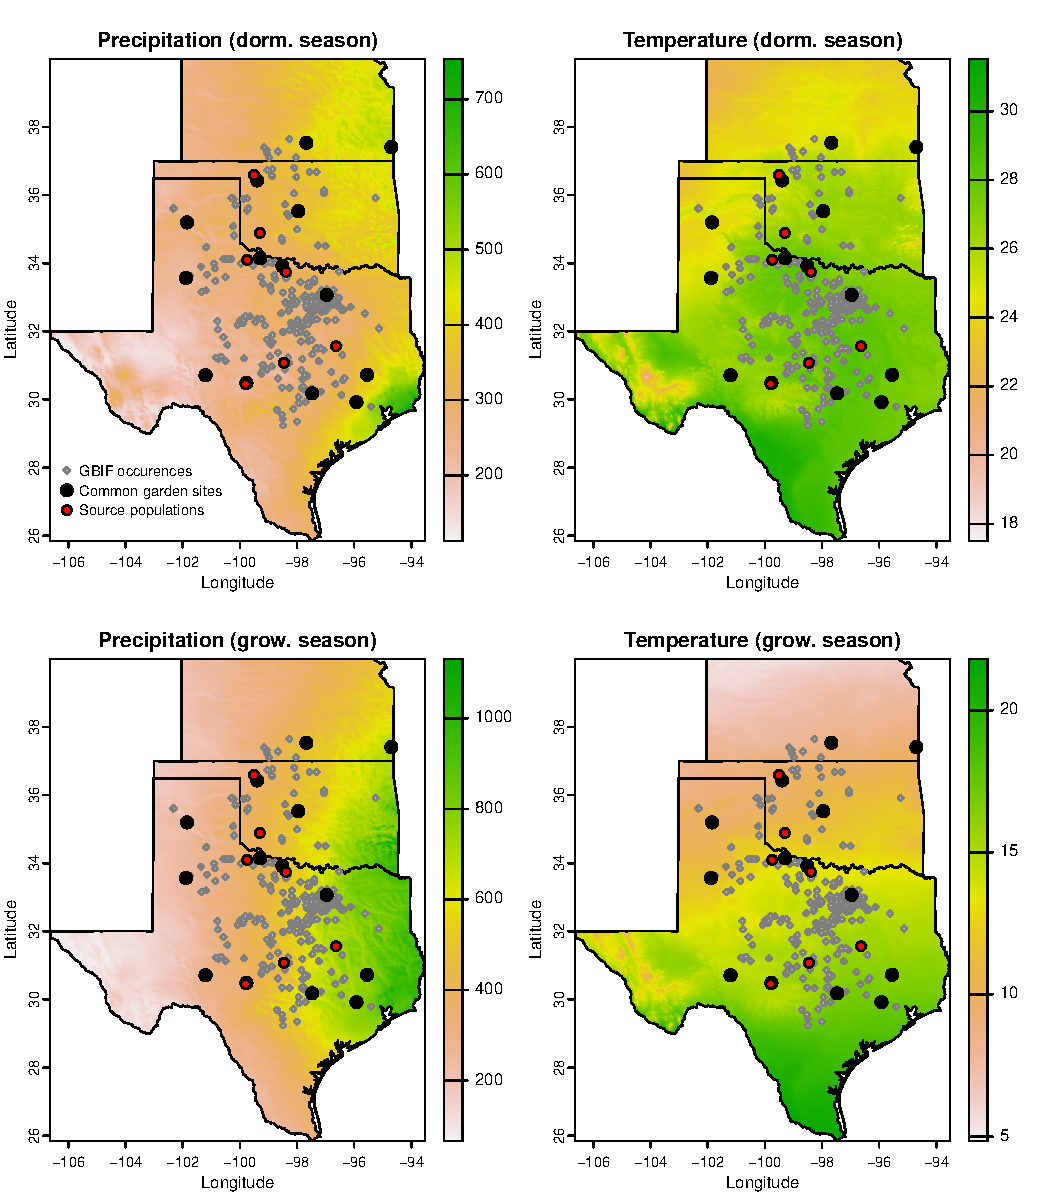
\includegraphics[width=0.90\linewidth]{Figures/POAR_survey_garden_map.pdf}
  \caption{\textbf{Maps of 30-year (1990-2019) normal climate and study sites used for demographic monitoring of \emph{Poa arachnifera} in Texas, Kansas and Oklahoma in the United States}.
  (A) Precipitation of the dormant season in mm , (B) temperature of the dormant season in \degree C , (C) precipitation of the growing season in mm , (D) temperature of the growing season in \degree C . 
  We surveyed 22 natural populations (grey diamond).
  The common garden sites were installed on 14 sites (black circle) collected from 7 sources populations (red circle). 
  Average temperatures along the distribution of the species tend to decrease northward as a result of the influence of latitude: lower latitudes receive more heat from the sun over the course of a year. 
  Similarly, the average precipitation decreases eastward as a result of the influence of longitude:  lower longitudes receive less precipitation over the year.
  See also Fig.\ref{Sup:pr_variation}, Fig.\ref{Sup:temp_variation}.}
  \label{fig:study_design}
  \end{center}
\end{figure}

\subsection*{Climatic data collection}
We downloaded monthly temperature and precipitation from Chelsa to describe observed climate conditions during our study period \citep{karger2017climatologies}.
These climate data were used as covariates in vital rate regressions, which allowed us to forecast and back-cast demographic responses to climate change based on observations across the common garden experiment. 
%We prefer temperature and precipitation because they capture the most the climate in the study region \colorbox{BurntOrange}{Source}. 
We aligned the climatic years to match demographic transition years {\color{blue}(May 1 -- April 30)} rather than calendar years.
Based on the natural history of this summer-dormant cool-season species, we divided each transition year into growing and dormant seasons. 
We define June through September as the dormant season and the rest of the year as the growing season. 
Across years and sites, the experiment included substantial variation in growing and dormant season temperature and precipitation (Fig. \ref{Sup:pr_variation}, \ref{Sup:temp_variation}).

To back-cast and forecast changes in climate, we downloaded projection data for three 30-year periods: past (1901-1930), current (1990-2019) and future (2070-2100).
Data for these climatic periods were downloaded from four general circulation models (GCMs) selected from the Coupled Model Intercomparison Project Phase 5 (CMIP5). 
The GCMs are: Model for Interdisciplinary Research on Climate (MIROC5), Australian Community Climate and Earth System Simulator (ACCESS1-3), Community Earth System Model (CESM1-BGC), Centro Euro-Mediterraneo sui Cambiamenti Climatici Climate Model (CMCC-CM).
All the GCMs were downloaded from chelsa \citep{sanderson2015representative}.
We evaluated future climate projections from two scenarios of representative concentration pathways (RCPs): RCP4.5, an intermediate-to-pessimistic scenario assuming a radiative forcing to amount to 4.5 $W m^{-2}$ by 2100, and RCP8.5, a pessimistic emission scenario which project a radiative forcing to amount to 8.5 $W m^{-2}$ by 2100 \citep{thomson2011rcp4, schwalm2020rcp8}.

\subsection*{Sex ratio experiment}
We conducted a sex-ratio experiment on a site close (1 km) to a natural population of the focal species at the center of the range to estimate the effect of sex-ratio variation on female reproductive success.
Details of the experiment are provided in \cite{compagnoni2017can} and \cite{miller2022two}.
In short, we established 124 experimental populations on plots measuring 0.4 x 0.4m and separated by at least 15m from each other at that site. 
We chose 15m because our pilot data show that more than 90\% of wind pollination occurred within 13m. 
We varied population density (1-48 plants/plot) and sex ratio (0\%-100\% female) across the experimental populations, and we replicated 34 combinations of density-sex ratios. 
We collected the number of panicles from a subset of females in each plot and collected the number of seeds in each panicle.
Since the number of panicles (proxy of reproduction effort) does not necessarily reflect reproduction success in \textit{Poar arachnifera}, we accessed reproduction success (seed fertilized) using greenhouse-based germination and trazolium-based seed viability assays. 

We used the sex-ratio to estimate the probability of viability and the germination rate. 
Seed viability was modeled with a binomial distribution where the probability of viability ($v$) was given by:
\begin{align}\label{eq:viab_fn}
v = v_{0} * (1 - OSR^{\alpha})
\end{align}
\noindent where $OSR$ is the operational sex ratio (proportion of panicles that were female) in the experimental populations.
The properties of the above function is supported by our previous work \citep{compagnoni2017can}. 
Here, seed viability is maximized at $v_{0}$ as $OSR$ approaches zero (strongly male-biased) and goes to zero as $OSR$ approaches $1$ (strongly female-biased).
Parameter $\alpha$ controls how viability declines with increasing female bias.

We used a binomial distribution to model the germination data from greenhouse trials.
Given that germination was conditional on seed viability,the probability of success was given by the product $v*g$, where $v$ is a function of $OSR$ (Eq. \ref{eq:viab_fn}) and $g$ is assumed to be constant.

\subsection*{Sex specific demographic responses to climate}
We used individual level measurements of survival, growth (number of tillers), flowering, number of panicles to independently develop Bayesian mixed effect models describing how each vital rate varies as a function of sex, size, precipitation of growing and dormant season and temperature of of growing and dormant season. 
We fit vital rate models with second-degree polynomial functions for the influence of climate.
We included a second-degree polynomial because we expected that climate variables would affect vital rates through a hump-shaped relationship. 

We centered and standardized all climatic predictors to facilitate model convergence.
However, Size was on a natural logarithm scale. 
We included site,source, and block as random effect.
All the vital rate models used the same linear and quadratic predictor for the expected value ($\mu$)(Eq.\ref{eq:mu}) . 
However, we applied a different link function ($f(\mu)$) depending on the distribution the vital rate. 
We modeled survival and flowering data with a Bernoulli distribution.
We modeled the growth (tiller number) with a zero-truncated Poisson inverse Gaussian distribution. 
Fertility (panicle count) was model as zero-truncated negative binomial. 
\begin{align}\label{eq:mu}
\begin{split}
\mu = \beta_{0} + \beta_{1}size + \beta_{2}sex + \beta_{3}pptgrow + \beta_{4}pptdorm + \beta_{5}tempgrow + \beta_{6}tempdorm \\ 
+ \beta_{7}pptgrow*sex + \beta_{8}pptdorm*sex + \beta_{9}tempgrow*sex + \beta_{10}tempdorm*sex  \\ 
+  \beta_{11}size*sex + \beta_{12}pptgrow*tempgrow + \beta_{13}pptdorm*tempdorm\\
+ \beta_{14}pptgrow*tempgrow*sex + \beta_{15}pptdorm*tempdorm*sex + \beta_{16}pptgrow^2\\
+ \beta_{17}pptdorm^2 + \beta_{18}tempgrow^2 + \beta_{19}tempdorm^2 + \beta_{20}pptgrow^2*sex  \\
+ \beta_{21}pptdorm^2*sex + \beta_{22}tempgrow^2*sex + \beta_{23}tempdorm^2*sex + \phi + \rho + \nu 
\end{split}
\end{align}
\noindent where $\beta_{0}$ is the  grand mean intercept, $\beta_{1}$ is the size dependent slopes.
$size$ was on a natural logarithm scale. 
$\beta_{2}$...$\beta_{13}$ represent the climate dependent slopes.
$\beta_{14}$...$\beta_{23}$ represent the sex-climate interaction slopes.
$pptgrow$ is the precipitation of the growing season (standardized to mean zero and unit variance), $tempgrow$ is the temperature of the growing season (standardized to mean zero and unit variance), $pptdorm$ is the precipitation of the dormant season (standardized to mean zero and unit variance), $tempdorm$ is the temperature of the dormant season (standardized to mean zero and unit variance).
The model also includes normally distributed random effects for block-to-block variation ($\phi \sim N(0,\ \sigma_{block})$) and source-to-source variation that is related to the provenence of the seeds used to establish the common garden ($\rho \sim N(0,\ \sigma_{source})$), site to site variation ($\nu \sim N(0,\ \sigma_{site})$).
We fit survival, growth, flowering models with generic weakly informative priors for coefficients ($\mu = 0,\ \sigma = 1.5$) and variances ($\gamma [0.1,\ 0.1]$).
We fit fertility model with regularizing priors for coefficients ($\mu = 0,\ \sigma = 0.15$).
% because the models could not converge with the same priors that was used for he other vital rates.
We ran three chains for 1000 samples for warmup and 4000 for interactions, with a thinning rate of 3.
We accessed the quality of the models using trace plots and predictive check graphs \citep{piironen2017comparison} (Fig. \ref{Sup:PPC}).
To understand the effect of climate on vital rates, we got the 95 \% credible interval of the posterior distribution.  
Then we assumed that there is 95 \% probability that the true (unknown) estimates would lie within that interval, given the evidence provided by the observed data for each vital rate.
All models were fit in Stan \citep{rstan}. 

\subsection*{Influence of climate variation on population growth rate}
To understand the effect of climate on population growth rate, we used the vital rate estimated earlier to build a matrix projection model (MPM) structured by size (number of tillers), sex and climate (dormant and growing) as covariate.  
Let $F_{x,z,t}$ and $M_{x,z,t}$ be the number of female and male plants of size $x$ in year $t$ present at a location that has $z$ as climate, where $x \in \{1,2,...,U\}$ and $U$ is the maximum number of tillers a plant can reach (here 95th percentile of observed maximum size).
Let $F^{R}_{t}$ and $M^{R}_{t}$ be the new recruits, which we assume do not reproduce in their first year.
We assume that the parameters of sex ratio-dependent mating (Eq. \ref{eq:viab_fn}) do not vary with climate.  
For a pre-breeding census, the expected numbers of recruits in year $t+1$ is given by:
\begin{align}\label{eq:recruits}
F^{R}_{t+1} = \sum_{x=1}^{U} 	[ \, p^{F}(x,z) \cdot c^{F}(x,z) \cdot d \cdot v(\mathbf{F_{t}},\mathbf{M_{t}}) \cdot m \cdot \rho 	] \, F_{x,z,t}
\\
M^{R}_{t+1} = \sum_{x=1}^{U} 	[ \, p^{F}(x,z) \cdot c^{F}(x,z) \cdot d \cdot v(\mathbf{F_{t}},\mathbf{M_{t}}) \cdot m \cdot (1-\rho) 	] \, F_{x,z,t}
\end{align}

\noindent where $p^{F}$ and $c^{F}$ are flowering probability and panicle production for females of size $x$, $d$ is the number of seeds per female panicle, $v$ is the probability that a seed is fertilized, $m$ is the probability that a fertilized seed germinates, and $\rho$ is the primary sex ratio (proportion of recruits that are female), $z$ is the climate. 
Seed fertilization depends on the OSR of panicles (following Eq. \ref{eq:viab_fn}) which was derived from the $U \times 1$ vectors of population structure $\mathbf{F_{t}}$ and $\mathbf{M_{t}}$:
\begin{align}\label{eq:viab_MPM}
v(\mathbf{F_{t}},\mathbf{M_{t}}) = v_{0} * \left[ 1 - \left( \frac{\sum_{x=1}^{U} p^{F}(x,z) c^{F}(x,z) F_{x,z,t}}{\sum_{x=1}^{U} p^{F}(x,z) c^{F}(x,z) F_{x,z,t} + p^{M}(x,z) c^{M}(x,z) M_{x,z,t}} \right) ^{\alpha}\right]
\end{align}

Thus, the dynamics of the size-structured component of the population are given by:
\begin{align}\label{eq:dynamics}
F_{y,t+1} = [ \, \sigma \cdot g^{F}(y,x=1,z) ] \, F^{R}_{t} + \sum_{x=1}^{U} 	[ \, s^{F}(x,z) \cdot g^{F}(y,x,z)] \, F_{x,z,t}
\\
M_{y,t+1} = [ \, \sigma \cdot g^{M}(y,x=1,z) ] \, M^{R}_{t} + \sum_{x=1}^{U} 	[ \,  s^{M}(x,z) \cdot g^{M}(y,x,z) ] \, M_{x,z,t}
\end{align}

\noindent In the two formula above, the first term indicates seedlings that survived their first year and enter the size distribution of established plants.
Instead of using \textit{P. arachnifera} survival probability, we used the seedling survival probability ($\sigma$) from demographic studies of the hermaphroditic congener \textit{Poa autumnalis} in east Texas (T.E.X. Miller and J.A. Rudgers, \textit{unpublished data}), and we assume this probability was constant across sexes and climatic variables. 
We did this because we had little information on the early life cycle transitions of greenhouse-raised transplants.
We also assume that $g(y,x=1)$ is the probability that a surviving seedlings reach size $y$, the expected future size of 1-tiller plants from the transplant experiment.
The second term represents survival and size transition of established plants from the previous year, where $s$ and $g$ give the probabilities of surviving at size $x$ and growing from sizes $x$ to $y$, respectively, and superscripts indicate that these functions may be unique to females ($F$) and males ($M$).

Since the two-sex MPM is nonlinear (vital rates affect and are affected by population structure) we estimated the asymptotic geometric growth rate ($\lambda$) by numerical simulation, and repeated this across a range of climate.

\subsection*{Identifying the mechanisms of population growth rate sensitivity to climate }
To identify which aspect of climate is most important for population viability, we used a "random design" Life Table Response Experiment (LTRE). 
We used the RandomForest package to fit a regression model with seasonal climate (here $\theta$) as predictors  and $\lambda$ as response \citep{ellner2016data,liaw2002classification}.
The LTRE approximates the variation in $\lambda$ in response to seasonal climate covariates and their interaction \citep{caswell2000matrix,hernandez2023exact}:
\begin{align}\label{eq:ltre}
Var(\lambda_{c})\approx \sum_{i=-1}^{n}\sum_{j=1}^{n} Cov(\theta_{i},\theta_{j},\theta_{ij}) + Var (\epsilon)
\end{align}

\noindent where, $\theta_{i}$, $\theta_{j}$, $\theta_{ij}$  represent respectively the fitted regression slope for the covariates of the dormant season,j the covariates of the growing season and ij the covariates of their interactions. 

To identify the mechanism by which climate affects population growth rate for each sex, we decomposed the effect of each climate variable on population growth rate ($\lambda$) into contribution arising from the effect on each stage-specific vital rate \citep{caswell2000matrix}.
At this end we used another LTRE with a "regression design". 
The LTRE with a "regression design" approximates the change in $\lambda$ with climate as the product of the sensitivity of $\lambda$ to the parameters times the sensitivity of the parameters to climate, summed over all parameters \citep{caswell1989analysis}:
\begin{align}\label{eq:ltresex}
\frac{\partial \lambda}{\partial climate} \approx \sum_{i} \frac{\partial \lambda}{\partial \theta^{F}_{i}} \frac{\partial \theta^{F}_{i}}{\partial climate} + \frac{\partial \lambda}{\partial \theta^{M}_{i}} \frac{\partial \theta^{M}_{i}}{\partial climate}
\end{align}

\noindent where, $\theta^{F}_{i}$ and $\theta^{M}_{i}$ represent sex-specific parameters: the regression coefficients for the intercepts and slopes of size-dependent vital rate functions. 
Because LTRE contributions are additive, we summed across vital rates to compare the total contributions of female and male parameters. 

\subsection*{Impact of climate change on niche and range shifts}
A species' ecological niche can be defined as the range of resources and conditions allowing its populations to self- sustained  ($\lambda > 1$) \citep{maguire1973niche,hutchinson1978introduction}.
To understand the impact of climate change on species niche shifts, we estimated the probability of self- sustaining populations, which is Pr ($\lambda > 1$) conditional to two environmental axes: (i) temperature and precipitation of the dormant season and (ii) temperature and precipitation of the growing season. 
Pr ($\lambda > 1$) was calculated using the proportion of the 300 Markov chain Monte Carlo iterations that lead to a $\lambda > 1$ \citep{diez2014probabilistic}.

Pr ($\lambda > 1$) was also mapped onto geographic layers of three state (Texas, Oklahoma and Kansas) to delineate past, current and future potential distribution of the species.
To do so, we estimated Pr ($\lambda > 1$) conditional to all climate covariates for each pixel ($\sim$340 km2) across the species range. 
Then we add the current occurrences record of the species (1990-2019) from Global Biodiversity Information Facility (GBIF) to validate the accuracy of our prediction
Because of the amount of the computation involve in the Markov chain Monte Carlo iterations, use only 100 posterior samples to estimate Pr ($\lambda > 1$) across the Texas, Oklahoma and Kansas.

All the analysis were performed in R 4.3.1 \citep{RCoreteam}
However the estimation of the impact of climate change on niche and range shifts were processed in parallel using open-source software on the Rice Super computer (NOTS) and the German Centre for Integrative Biodiversity Research (iDiv) High-Performance Computing Cluster.

\section*{Results}
\subsection*{Sex specific demographic response to climate change}
Most vital rates were strongly climate dependent, but the magnitude of their response were similar between sexes suggesting no sex-specific demographic response to climate. 
Survival and flowering were strongly more dependent on climate than growth (number of tillers) and reproduction (number of panicles) (Fig.\ref{fig:vital_rates}; Fig. \ref{Sup:Posterior}).
In addition, we found opposite patterns in the direction of the effect on seasonal climate on the probability of survival and flowering.
The growing season (precipitation) has a negative effect on the probability of survival, number of tillers, and the probability of flowering, whereas the dormant season has a positive effect on these vital rates. 
Unlike precipitation, temperature of the growing season has a positive effect of the probability of survival, a negative effect of the probability of flowering, and the number of tillers, but no significant effect on the number of panicles. 
Further, there was a female survival and flowering advantage across both climatic seasons (Figures. 3A-3D, 3I-3L). 
On the contrary, there was a male panicle advantage across all climatic variables (Figure3M-3P). 
Counter-intuitively, there was no significant sex growth advantage in all season climatic variables (Figures. 3E-3H). 
% Plant size and sex interaction was significant for all vitals rates (Fig. \ref{Sup:Posterior}), suggesting a sexual dimorphism.
% For survival, flowering and reproduction the interaction between temperature and precipitation of the growing season and dormant season was not significant (Fig. \ref{Sup:Posterior}). 
% However, for growth, the interaction between temperature and precipitation of the growing season and dormant season was significantly higher than zero (Fig. \ref{Sup:Posterior}). 

\begin{figure}[H]
  \begin{center}
    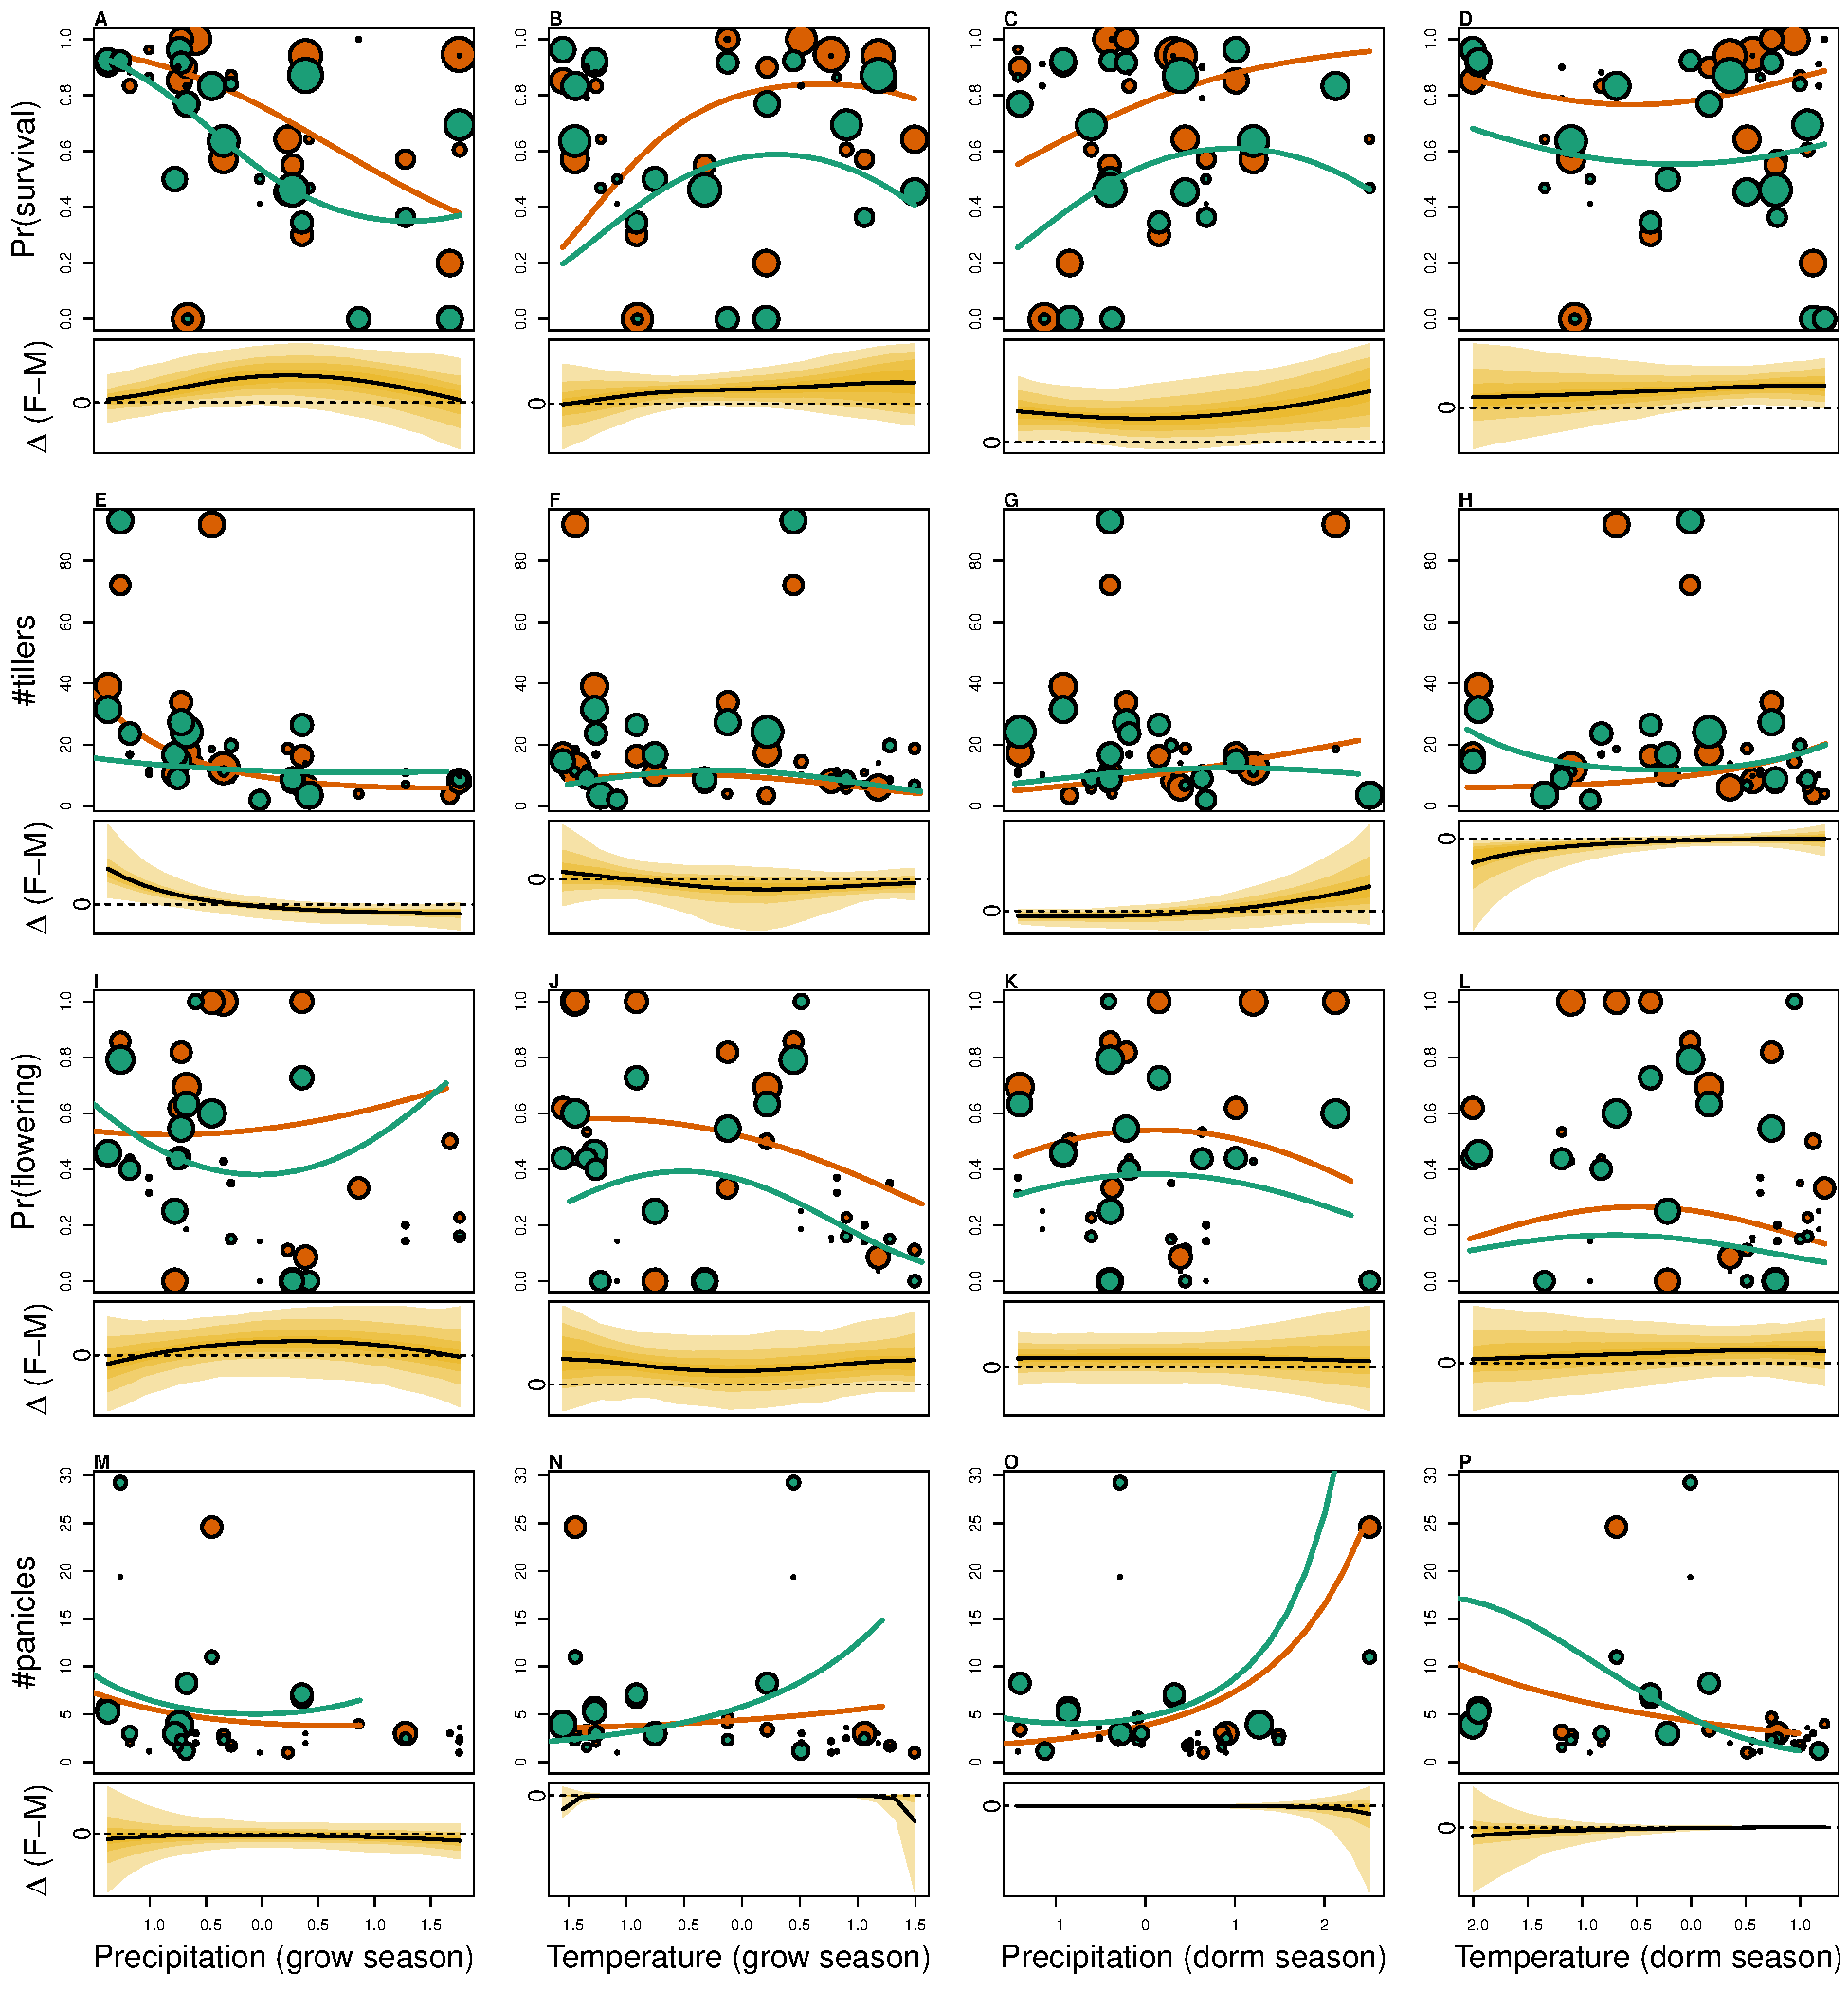
\includegraphics[width=0.95\linewidth]{Figures/vital_rates.pdf}
  \caption{\textbf{Sex specific demographic response to climate across species range}.
  (A, B) Probability of survival during the growing season; (C, D) Probability of survival during the dormant season
  (E, F) Change in number of tillers during the growing season; (F, G) Change in number of tillers during the dormant season
  (I, J), Probability of flowering during the growing season; (K, L) Probability of flowering during the dormant season
  (M, N), Change in number of panicles produced given flowering during the growing season; (O, P) Change in number of panicles produced given flowering during the dormant season.
  Points show means by site for females (orange) and males (green). 
  Points sizes are proportional to the sample sizes of the mean and are jittered.
  Lines show fitted statistical models for females (orange) and males (green) based on posterior mean parameter values.
  Lower panels below each data panel show the posterior distribution of the difference between females and males as a function of climate (positive and negative values indicate female and male advantage, respectively); dashed horizontal line shows zero difference.
  Statistical results are shown in Fig. \ref{Sup:Posterior}.}
  \label{fig:vital_rates}
  \end{center}
\end{figure}


\subsection*{Climate change alters population viability}
We estimated population growth rate response to seasonal climate gradients using two models: a female dominant model and a two-sex model. 
Consistent with the effect of climate on the individual vital rate, we found a strong effect of seasonal climate on population fitness (Fig.\ref{fig:lambda}). 
For both models, population growth rate decreased toward high precipitation of growing season (Fig.\ref{fig:lambda} A, C). 
In contrast population growth rate increased with an increase in precipitation of the dormant season.
Furthermore, population growth rate was maximized between 14 and 17 \degree C and decreased bellow zero beyond 18 \degree C during the growing season (Fig.\ref{fig:lambda} B).
Similarly population fitness was maximized between 27 and 31 \degree C and decreasesd bellow zero just beyond 20 \degree C during the dormant season (Fig.\ref{fig:lambda} D).
% Across species niche population persistence was maximized at higher temperature during the dormant season ( 27 to 31) and intermediate temperature during the growing season (11 to 20).
We have also detected a strong effect of the past and future climate on population growth rate. 
However, the magnitude of the effect of future climate on population growth rate was different between gas-scenario emissions. 
Under past climate conditions, population growth rate decreased below one for temperature of the growing season.
A moderate emission gas scenario (RCP4.5) has a no effect on the population growth rate while a high emission scenario (RCP8.5) has a strong negative effect on population growth rate (Fig.\ref{fig:lambda} B, D). 

\begin{figure}[H]
  \begin{center}
    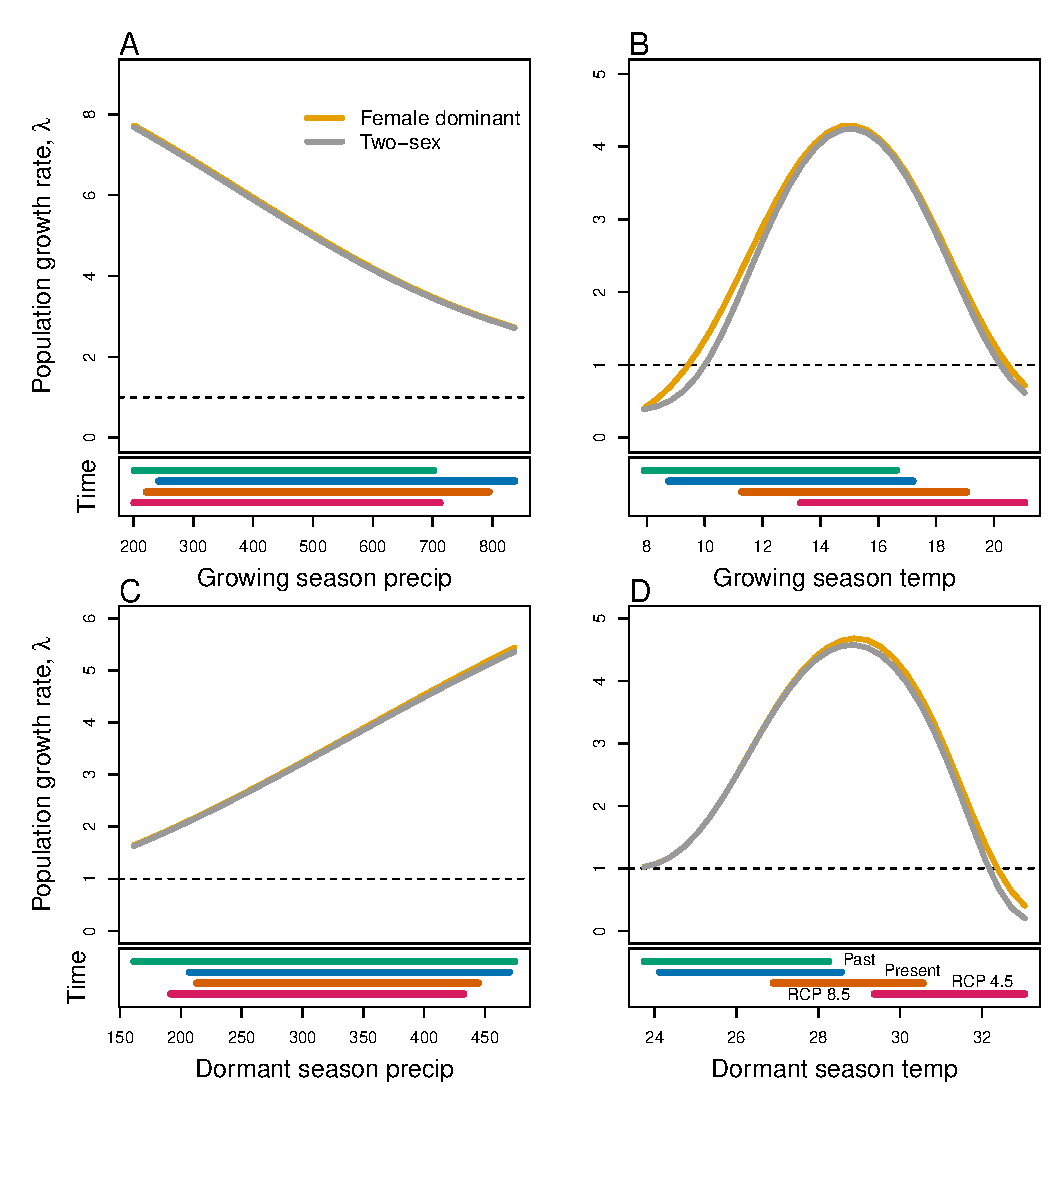
\includegraphics[width=0.85\linewidth]{Figures/lambda_past_present_future.pdf}
  \caption{\textbf{Population growth rate ($\lambda$) as a function of seasonal climate}.
(A) Precipitation of the growing season, (B) Temperature of the growing season, (C) Precipitation of the dormant season, (D) Temperature of the dormant season.
The grey curve shows prediction by the two-sex matrix projection model that incorporates sex- specific demographic responses to climate with sex ratio dependent seed fertilization.
The orange curve represents the prediction by the female dominant matrix projection model.
The dashed horizontal line indicates the limit of population viability ($\lambda$ = 1).
Lower panels below each data panel shows climate values at different time perdio (past climate, present and future climates).
For future climate, we show a Representation Concentration Pathways (RCP) 4.5 and 8.5. Values of ($\lambda$) are derived from the mean climate variables across 4 GCMs (MIROC5, ACCESS1-3, CESM1-BGC, CMCC-CM).}
  \label{fig:lambda}
  \end{center}
\end{figure}

\subsection*{Temperature as a driver of population growth rate decline }
Population growth rate was most sensitive to change in temperature of the growing season and temperature of the dormant season (Supporting Information \ref{Sup:LTRE}). 
LTRE decomposition revealed that, for each sex, the reduction of $\lambda$ for high value of temperature of the growing season was driven by a reduction of survival rate, growth rate, and a reduction in number of panicles (Fig.\ref{fig:LTRETemp} A, B). 
However, the reduction of population growth rate for higher value of temperature of the dormant season was driven by only female individuals(Fig.\ref{fig:LTRETemp} C, D). 
The increase of the probability of flowering was sufficient to prevent population growth rate from declining for high tmeprature of the dormant season (Fig.\ref{fig:LTRETemp} C).
\begin{figure}[H]
  \begin{center}
    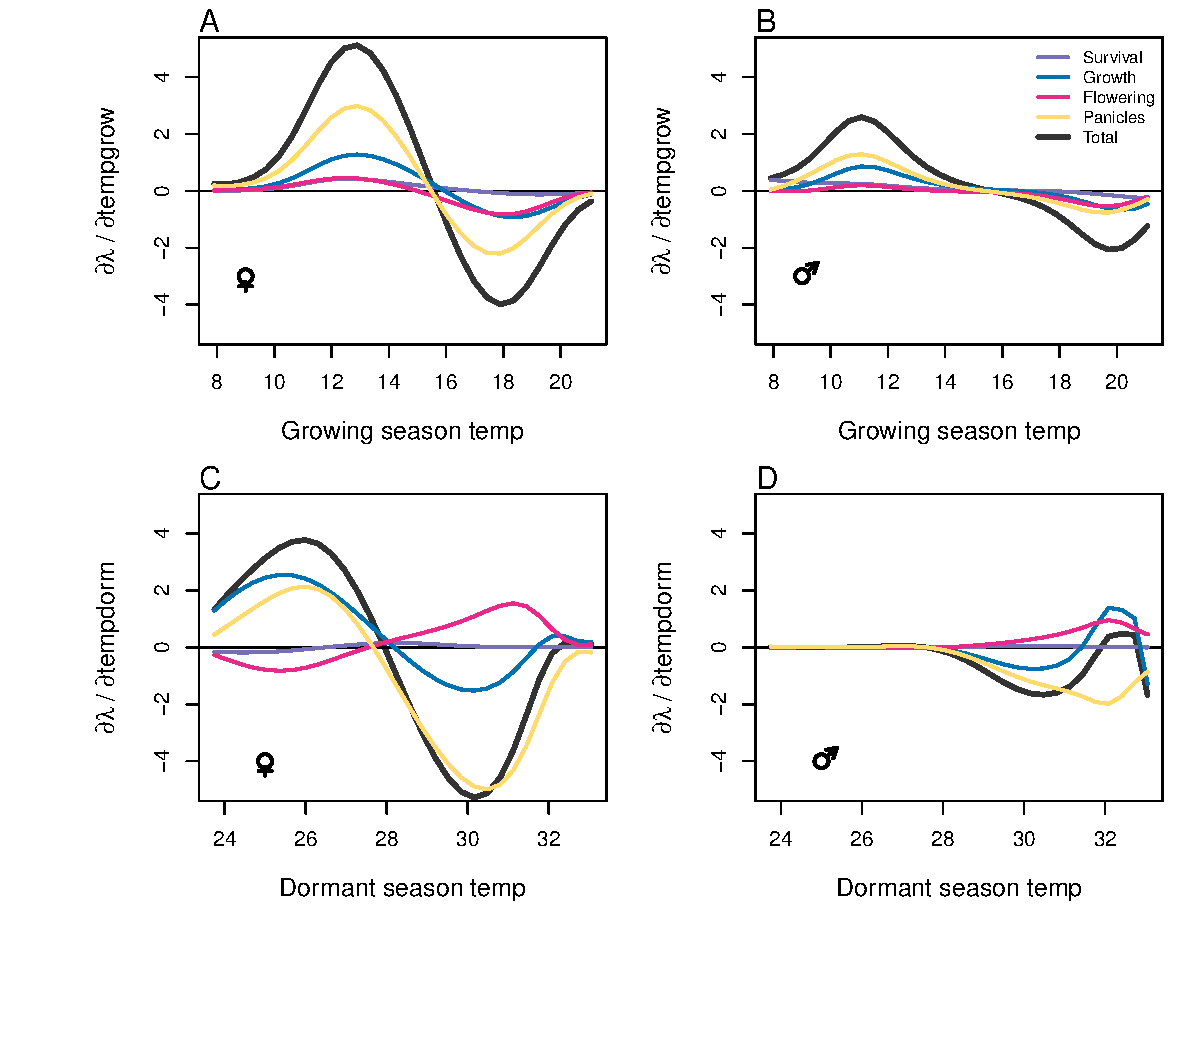
\includegraphics[width=0.85\linewidth]{Figures/LTRE_Temperature.pdf}
  \caption{\textbf{Life table response experiment decomposition of the sensitivity of $\lambda$ to seasonal climate into additive vital rate contributions of males and females based on posterior mean parameter estimates.}
 (A) Temperature of growing season (contribution of female), (B) Temperature of growing season (contribution of male),  (C) Temperature of dormant season (contribution of female) and (D) Temperature of dormant season (contribution of male).}
  \label{fig:LTRETemp}
  \end{center}
\end{figure}

\subsection*{Climatic change induce niche and range shifts}
Our results suggested niche sifts for both models (female dominant and two-sex) during the dormant and growing season (Fig. \ref{fig:niche}). 
However, the female dominant model overestimated the magnitude of niche shifts (Fig. \ref{fig:niche} D). 
Further, our demographically based range predictions broadly captured the known distribution of the species. 
More specifically, the predicted probabilities of self- sustaining ($\lambda>1$) matches the presence and absence of the species (Fig. \ref{fig:geoprojacc} B, Fig. \ref{fig:geoprojacc} F). 
Furthermore, viable populations of \emph{P. arichnifera} were only predicted at the center of the range for current climatic conditions (Fig. \ref{fig:geoprojacc} B).
Although \emph{P. arichnifera} was predicted to have suitable habitats in the center of the range under current climate, global  warming (regardless of the future scenario of carbon emission used) is predicted to reduce much of these suitable habitats (Fig. \ref{fig:geoprojacc} C, D). 
Most of the current suitable habitats will move toward the Northern range edge.  

\begin{figure}[H]
  \begin{center}
    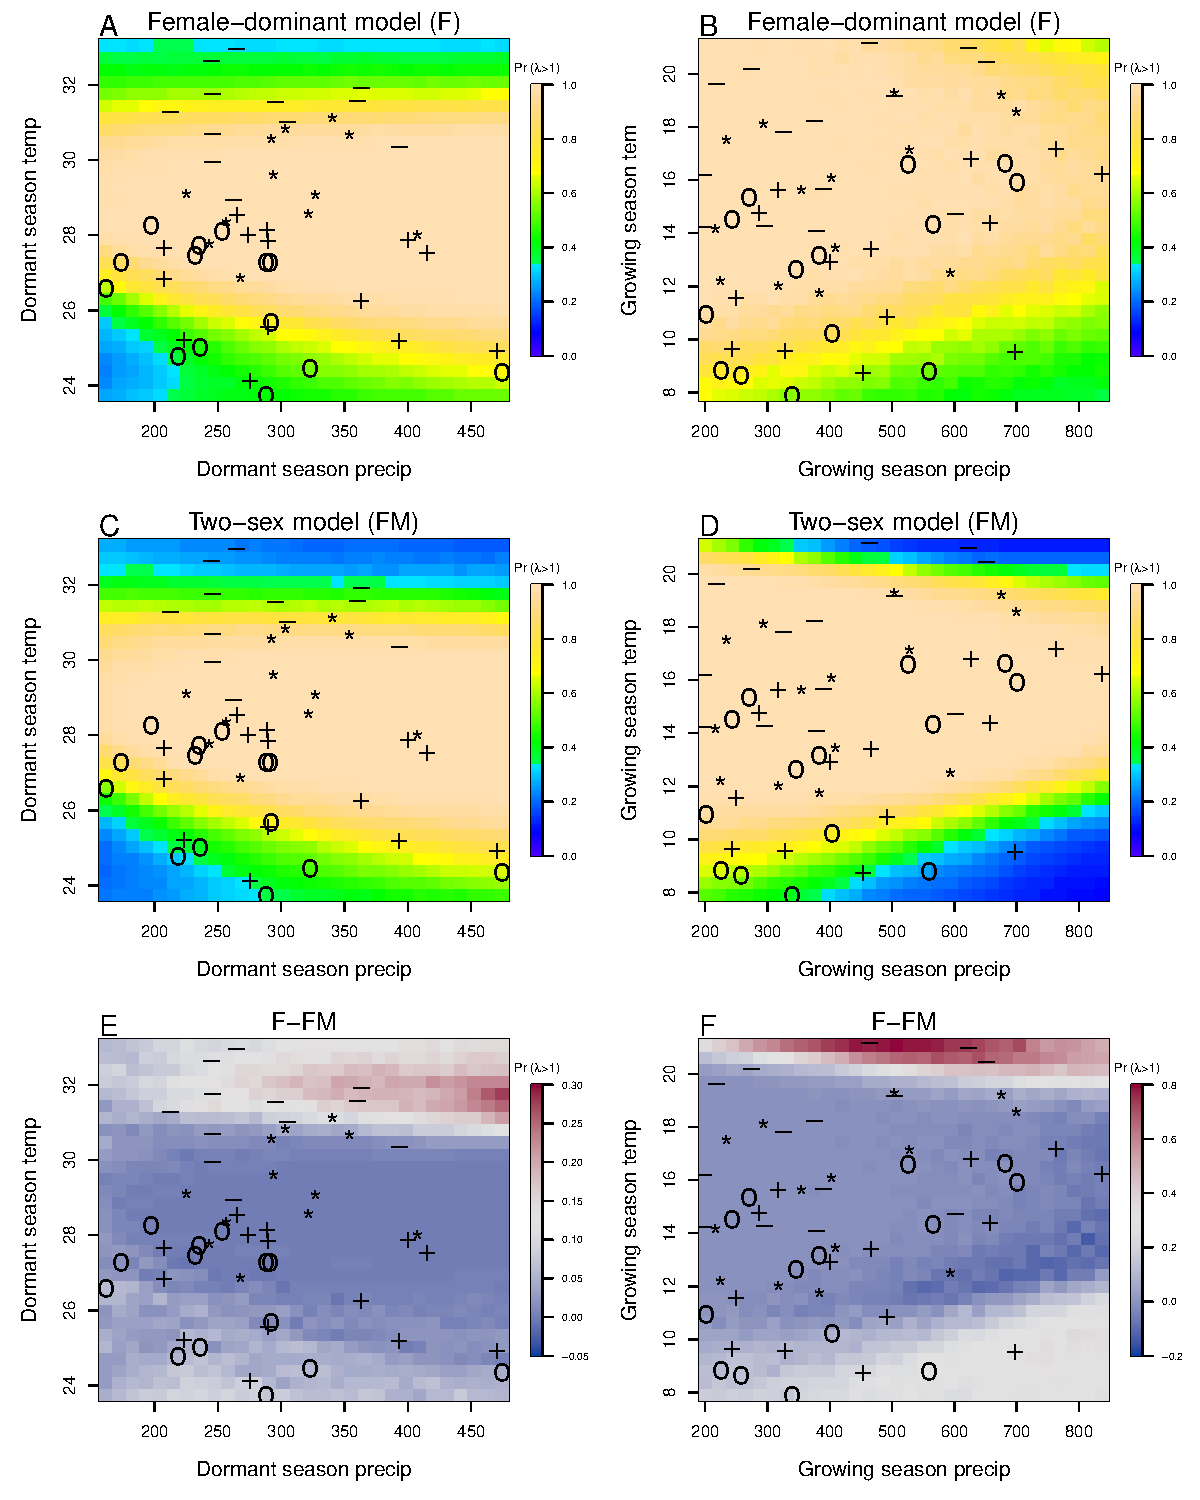
\includegraphics[width=0.85\linewidth]{Figures/niche_dormant_growing.pdf}
  \caption{\textbf{A two‐dimensional representation of the predicted niche shift over time (past, present and future climate conditions)}. 
  Contours show predicted probabilities of self- sustaining populations, Pr ($\lambda > 1$) conditional on precipitation and temperature of the dormant and growing season.
 (A) Niche of dormant season for the two sex model, (B) Niche of growing season for the two sex model,
 (C) Niche of dormant season for female dominant model, (D) Niche of growing season for female dominant model.
  "\begin{normalsize}\textbf{o}\end{normalsize}": Past, "\begin{normalsize}\textbf{+}\end{normalsize}": Current,"\begin{large}\textbf{*}\end{large}": RCP 4.5,"\begin{tiny}$\blacksquare$\end{tiny}": RCP 8.5.}
  \label{fig:niche}
  \end{center}
\end{figure}

\begin{figure}[H]
  \begin{center}
    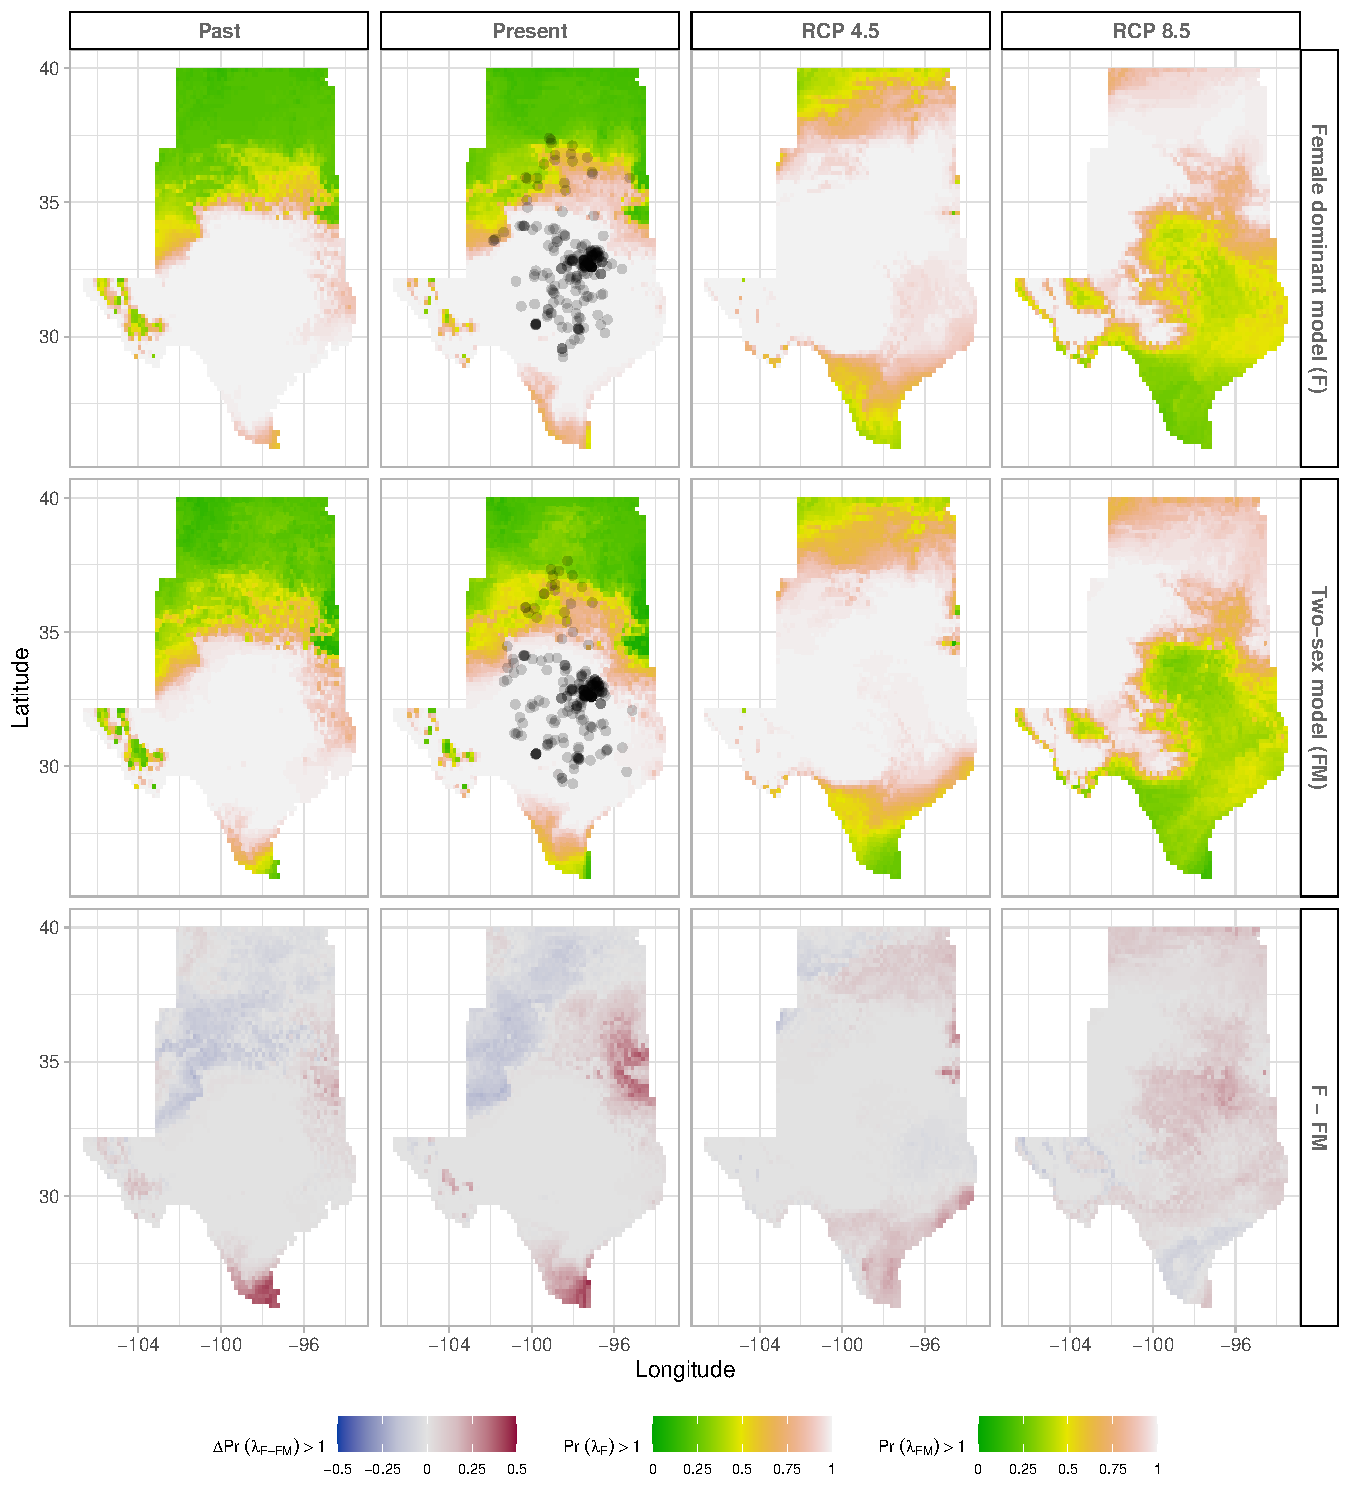
\includegraphics[width=0.99\linewidth]{Figures/Fig_geoPrlambdaacc.pdf}
  \caption{ \textbf{Climate change favors range shift toward the North edge of the current range.}
  (A) Past, (B) Current, (C and D) Future predicted range shift based on the predicted probabilities of self- sustaining populations, Pr ($\lambda > 1$), using the two-sex model that incorporates sex- specific demographic responses to climate with sex ratio dependent seed fertilization.
  (E) Past, (F) Current, (G and F) Future  predicted range shift based on the predicted probabilities of self- sustaining populations, Pr ($\lambda > 1$), using the female dominant model.
  Future projections were based on the ACCESS model.
  The black dots on panel B and F indicate all known presence points collected from GBIF from 1990 to 2019, which corresponds to the current condition in our prediction. 
  The occurrences of GBIFs are distributed in with higher population fitness habitat Pr ($\lambda$ > 1) , confirming that our study approach can reasonably predict range shifts. }
  \label{fig:geoprojacc}
  \end{center}
\end{figure}


\section*{Discussion}
Although much emphasis has been placed in the response of monoecious species to climate, we have little knowledge about how skewness in sex ratio will affect dioecious species population dynamics and dioecious range shifts. 
We forecasted range shifts in dioecious species using climate-demographic models. 
Three general patterns emerged from our analysis.
First, our Bayesian mixed effect model predicts that seasonal climate (temperature and precipitation) affects sex-demographic processes in distinctive and contrasting ways.
While climate has a significant effect on the probability of survival and growth, it has no effect on the number of panicles. 
Second, future climate, by increasing seasonal temperature, will reduce survival rate, growth rate and reproduction and thereby alter population viability.
In addition, climate change favors range shifts. 
Third, using only one sex to forescat range shifts of dioecious under climate change could lead to an overestimation of the impact of  climate change on species.

Our results indicate no sex-specific demographic response to climate change. 
However, females have higher survival rate and fertility rate than males. 
This result is not unique to our study system and has been observed in a range of pollen dispersal species across climatic gradients \citep{welbergen2008climate,zhao2012sex,sasaki2019complex}. 
Several hypotheses could explain the observed demographic advantage of females over males for survival and flowering and the opposite for growth and number of panicles.
The trade-off between fitness traits (survival, growth fertility) due to resource limitation and the pollination mode of our study species (wind pollinated) could explain such a result \citep{cipollini1994sexual,freeman1976differential}.
For most species, the cost of reproduction is often higher for females than males due to the requirement to develop seeds and fruits \citep{hultine2016climate}. 
However, several studies reported a higher cost of reproduction for males in wind pollinated species due to the larger amounts of pollen they produce \citep{burli2022environmental,cipollini1994sexual,bruijning2017surviving,field2013comparative}.
In addition to life history trade-off, difference in non-climatic factors such as soil, or biotic interactions could explain decline in vital rate as an indirect effects of increase in temperature \citep{alexander2015novel,schultz2022climate}.

Under current conditions, most populations across the range are viable.
This result could be explained by two hypotheses.
First, demographic compensation whereby an increase of one vital rate is coupled with a decrease of another vital rate could explain viable populations in harsh conditions at the range edge \citep{doak2010demographic,villellas2015demographic,nomoto2021drivers}. 
In our system, a decrease in fertility and survival rate was counterbalanced by an increase in flowering rate, preventing the population growth rate from declining even at range edge during the dormant season.
Second, local adaptation at the edge of the range could explain the viable populations throughout the range \citep{miller2022two}. 
Our study was based on a common garden experiment; therefore, individuals planted in climatic conditions that are similar to their source populations climatic conditions were less impacted by stressful environmental conditions.
An important question to ask is: what is the role of local adaptation in buffering species response against climate change.
Unfortunately, our model does not shed light on that question.
Adding another predictor to our complex model would have lead to overfitting. 
Therefore, the role of local adaptation in mitigating population response to climate should be the next step in forecasting species response to climate. 

Our LTRE analysis reveals that a small change in temperature of the growing and dormant season could have a larger  impact on population viability.
% This results corroborated with other studies and suggest that projected future climate will affect population viability \citep{reed2021climate}. 
Temperature can impact plant populations through different mechanisms. 
Increasing temperature could increase evaporative demand, affect plant phenology \citep{mclean2016predicting,sherry2007divergence,iler2019reproductive}, and germination rate \citep{reed2021climate}.
% In the  growing season, when the temperature is high, the effect on the water balance should be strong .
The potential for temperature to influence these different processes changes seasonally \citep{konapala2020climate}.
For example, studies suggested that species that are active during the growing season such as cool grass species can have delayed phenology in response to global warming, particularly if temperatures rise above their physiological tolerances \citep{cleland2007shifting,williams2015life}. 
In addition, high temperature during the growing season by affecting pollen viability, fertilization could affect seed formation and germination \citep{hatfield2015temperature,sletvold2015climate}. 
% Because our study species was sensitive to temperatures in the growing season, the former mechanism deserve further attention.
Temperature also affected operational sex ratio (OSR) (Fig.\ref{Sup:OSR}). 
That variation in OSR could affect population growth rate by altering females’ fitness \citep{petry2016sex,knight2005pollen,haridas2014frequency}. 

We found evidence of climatic niche shifts for the female dominant model and the two-sex model. 
However the female dominant model overestimated species niche, suggesting that using one sex to predict niche shifts could be misleading.
Despite that overestimation for the female dominant model, both models agree on the fact that climatic conditions that are not optimal under current conditions will be optimal for the species over the next years particularly at the edge of species. 
Further, pollen dispersal may allow plants to resist climate change because pollen dispersal may provide the local genetic diversity necessary to adapt at the leading edge of the population \citep{kremer2012long,corlett2013will,duputie2012genetic}.
Since wind pollination is most effective at short distances, it is most often found in plant species growing at high density such as our study species, it is less likely that dispersal limitation  affect niche shift in our study system. 
However, others biotic factors such as species competition might constrain the species to a narrower realized niche \citep{pulliam2000relationship,aguilee2016pollen}. 

Our results suggest that climate change will drive range shifts and the magnitude and rate of that range shift could be overestimated when tracking only one sex (Fig. \ref{Sup:geoprojces},Fig. \ref{Sup:geoprojcmc},Fig. \ref{Sup:geoprojmiroc}). 
This overestimation of the impact of climate change using a female dominant model could be do to several factors.
First, small change in seasonal temperature affects population viability for both sexes.
Second, operational sex ratio in \emph{Poa arachnifera} become female biased in area with lower temperature of growing season such as Northern range edge (Fig.\ref{Sup:OSR} B). 
Our results converge with previous studies that have found the same pattern for other dioecious species \citep{woldemelak2021effect,varga2020environmental}. 
Our funding also contrast with a previous study suggesting that an increase in male frequency induce range shifts by reducing pollen limitation in conditions that were not suitable \citep{petry2016sex}. 

Three years represent a relatively decent time for demographic study for common garden experiments across climatic gradient.
Thus our models can only capture a certain range of demographic and environmental variability (Fig. \ref{Sup:lambda2sex}).
Moreover, our future projections require extrapolation to warmer or colder conditions than observed in our experiment and subsequently should be interpreted with caution \citep{chen2024influence}. 
Despite all these limitations, the qualitative implications of a negative response of species to increase temperature (dormant and growing season) seems consistent across all GCMs.  
Most of the suitable areas move toward the North of the current range in response to climate change.
Climate change will affect population growth rate primarily through the response of female which is more sensitive to climate change \citep{miller2022two}.
Males also have a significant contribution to population growth rate particularly for temperature. 
Our work suggest that current climate may not affect population viability, but populations may be impacted negatively over the next decades in response to a climate change. 
This is key because most conservation actions are design from  data on current responses to climate, rather than future response to climate \citep{sletvold2013climate}. 
Moreover, management strategies that focus on both sex would be effective and will enhance population growth rate in response to global warming. 

\section*{Conclusion}
We have investigated the potential consequence of skewness in sex ratio on population dynamics and range shift in the context of climate change. 
We found that future climate will affect population growth rate at the center of species range.
This reduction in population growth rate will induce a range shift to the northern edge of the species current range. 
Our results also suggest that tracking only one sex could lead to an overestimation of the effect of climate change on population dynamics. 
Our work  provides a framework for predicting the impact of global warming on species using population demography. 

\section*{Acknowledgements}
We are thankful to Dariusz Malinowski, Jason Goldman, Tom Arsuffi, Alan Byboth, John Walker, Kenneth Steigman, Steven Gibson, Wesley Newman, Kerry Griffis, Liz Martin, Melanie Hartman, Brian Northup, Le-land Russell, Dexter R. Mardis, and Dixie Smith for facilitating our fieldwork. 
We acknowledge Marion Donald, Kory Kolis, Nakian Kim, and Alex Espana for valuable assistance in the field, laboratory, and greenhouse. 
We want also to acknowledge the network of biological field stations that hosted our geographically distributed experiment. 
We are also grateful to Sam Houston State University, Texas A\& M University, University of Texas, Texas Tech University, Pittsburgh State University, and Wichita State University for investing in field stations and making these facilities available to us. 
This research was supported by National Science Foundation Division of Environmental Biology awards 1543651 and 1754468 and by the Rice University Faculty Initiatives Fund.
This work was supported partially by the Big-Data Private-Cloud Research Cyberinfrastructure MRI-award funded by NSF under grant CNS-1338099 and by Rice University's Center for Research Computing (CRC).


\newpage
\bibliographystyle{apalike}
\bibliography{Forecasting}
%--------------------------------------------------------------------
\newpage
\clearpage 
\setcounter{equation}{0}
\setcounter{figure}{0}
\setcounter{section}{0}
\setcounter{table}{0}
\renewcommand{\theequation}{S.\arabic{equation}}
\renewcommand{\thetable}{S-\arabic{table}}
\renewcommand{\thefigure}{S-\arabic{figure}}
\renewcommand{\thesection}{S.\arabic{section}}

\centerline{\Large{\textbf{Supporting Information}}}

% \section {XX}	

\begin{figure}[H]
		\centering
		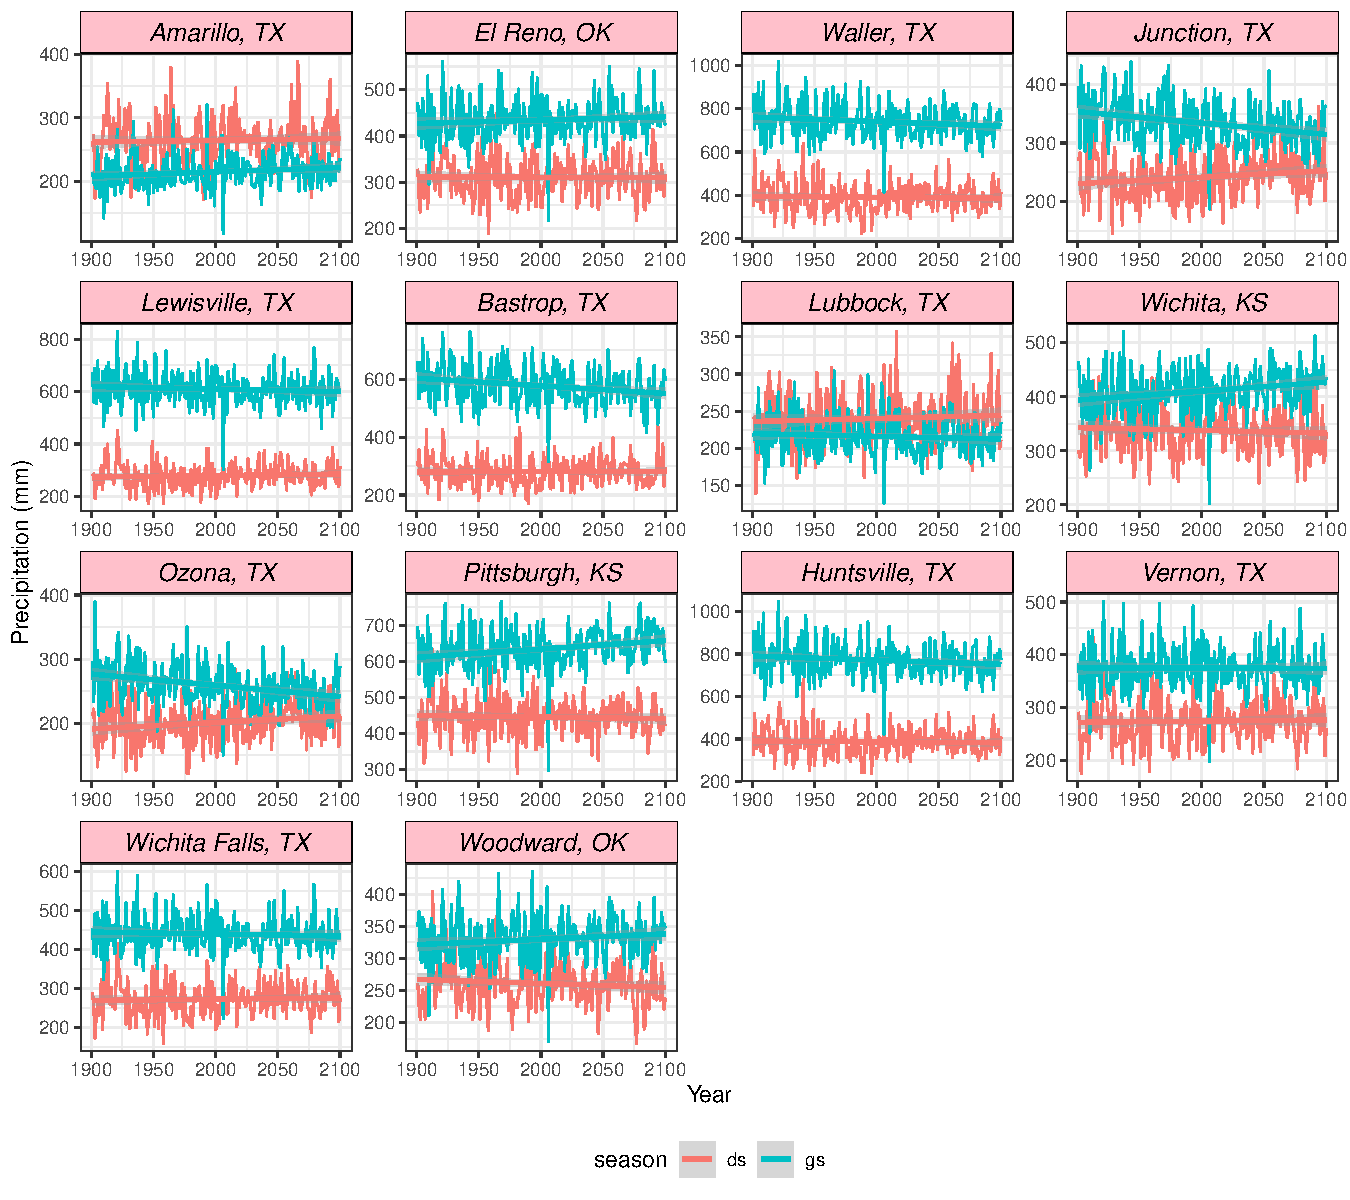
\includegraphics[width=0.95\linewidth]{Figures/fig_pr_past_present_future.pdf}
		\caption{Precipitation variation accross the study sites from 1990 to 2100.
		ds:Dormant season, dg:Growing season.}
		\label{Sup:pr_variation}
\end{figure}


\begin{figure}[H]
		\centering
		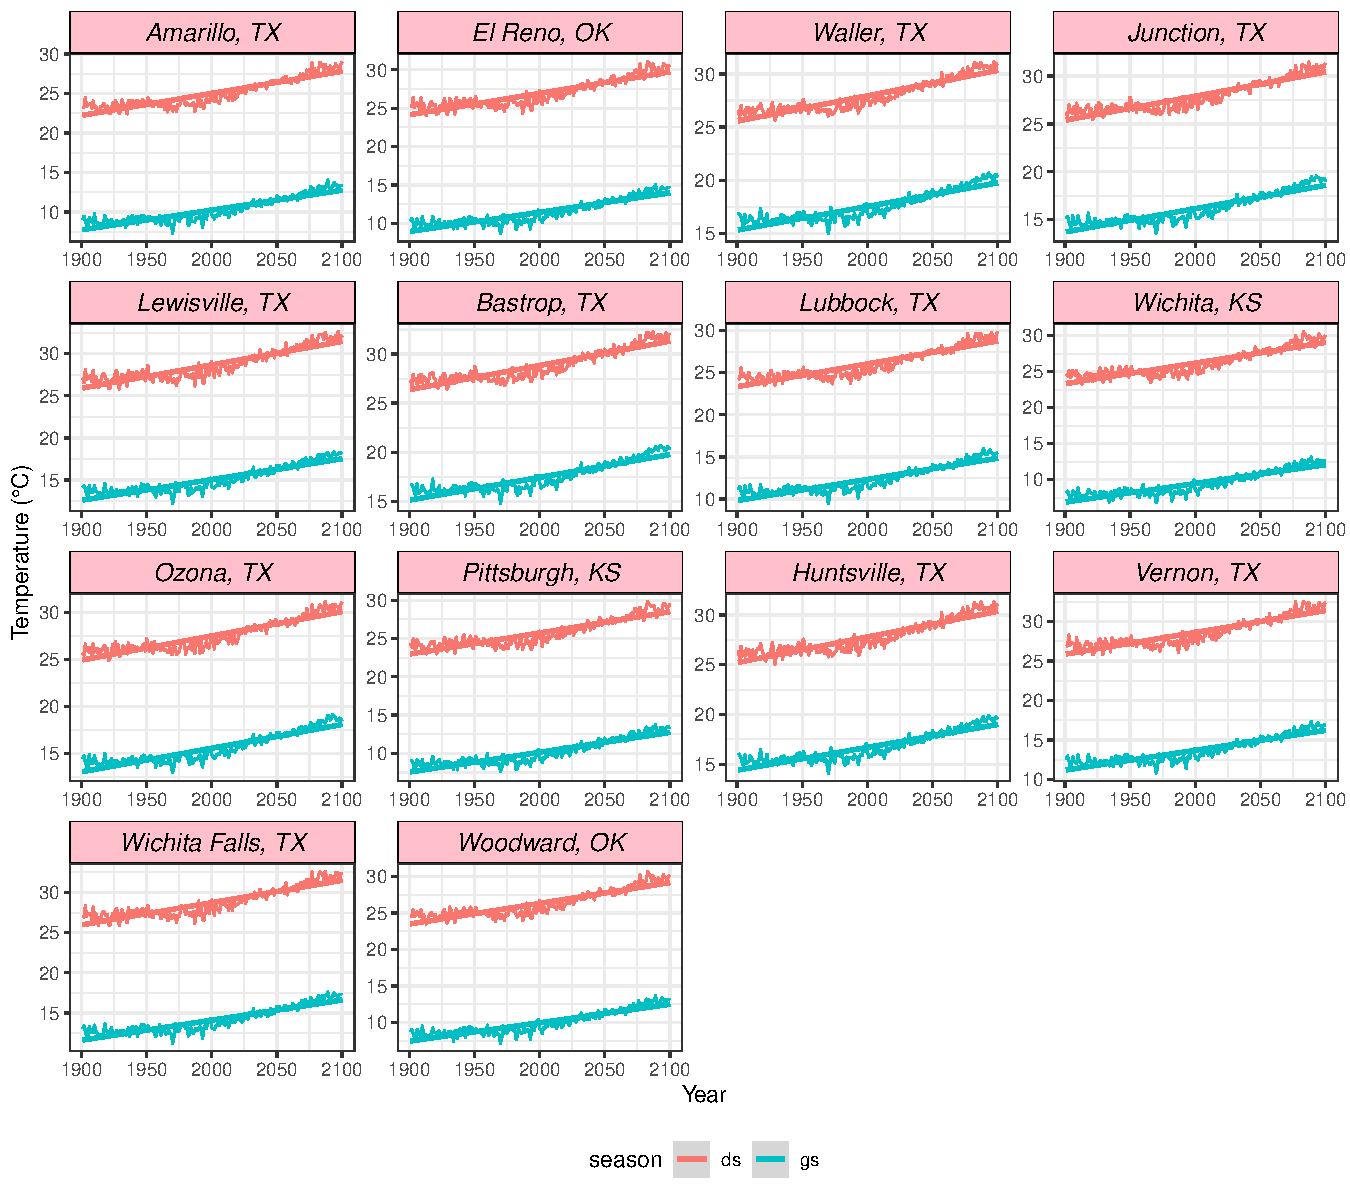
\includegraphics[width=0.95\linewidth]{Figures/fig_tas_past_present_future.pdf}
		\caption{Temperature variation accross the study sites from 1990 to 2100,
		ds: Dormant season, dg: Growing season.}
		\label{Sup:temp_variation}
\end{figure}

\begin{figure}[H]
		\centering
		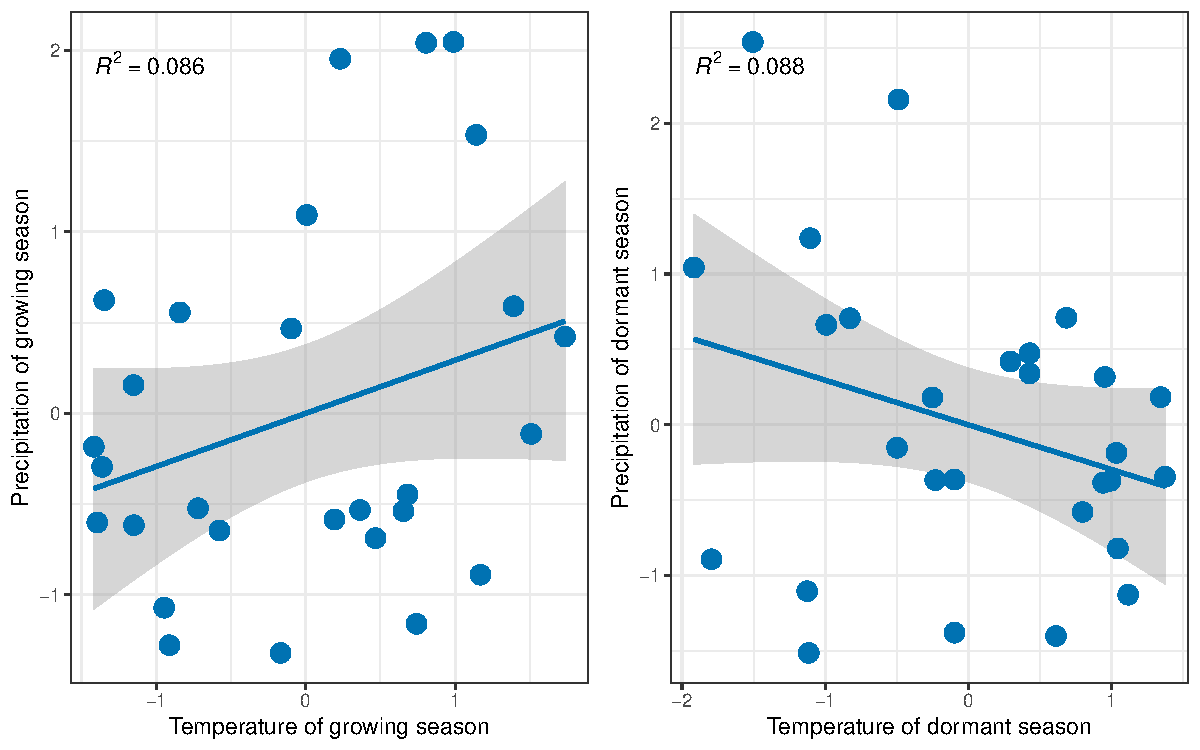
\includegraphics[width=0.95\linewidth]{Figures/Varianceexplained.pdf}
		\caption{Relation between precipitation and temperature for each season (growing and dormant). $R^2$ indicates the value of proportion of explained variance between the temperature and precipitation}
		\label{Sup:Correlation}
\end{figure}
	
\begin{figure}[H]
		\centering
		\includegraphics[width=0.75\linewidth]{Figures/PPC.pdf}
		\caption{Posterior predictive checks. Consistency between real data and simulated values suggests that the fitted model accurately describes the data. Graph shows density curves for the observed data (light blue ) along with the simulated values (dark blue). The first column shows the linear models and the second column shows the 2 degree polynomial models.}
		\label{Sup:PPC}
	\end{figure}
	
\begin{figure}[H]
		\centering
		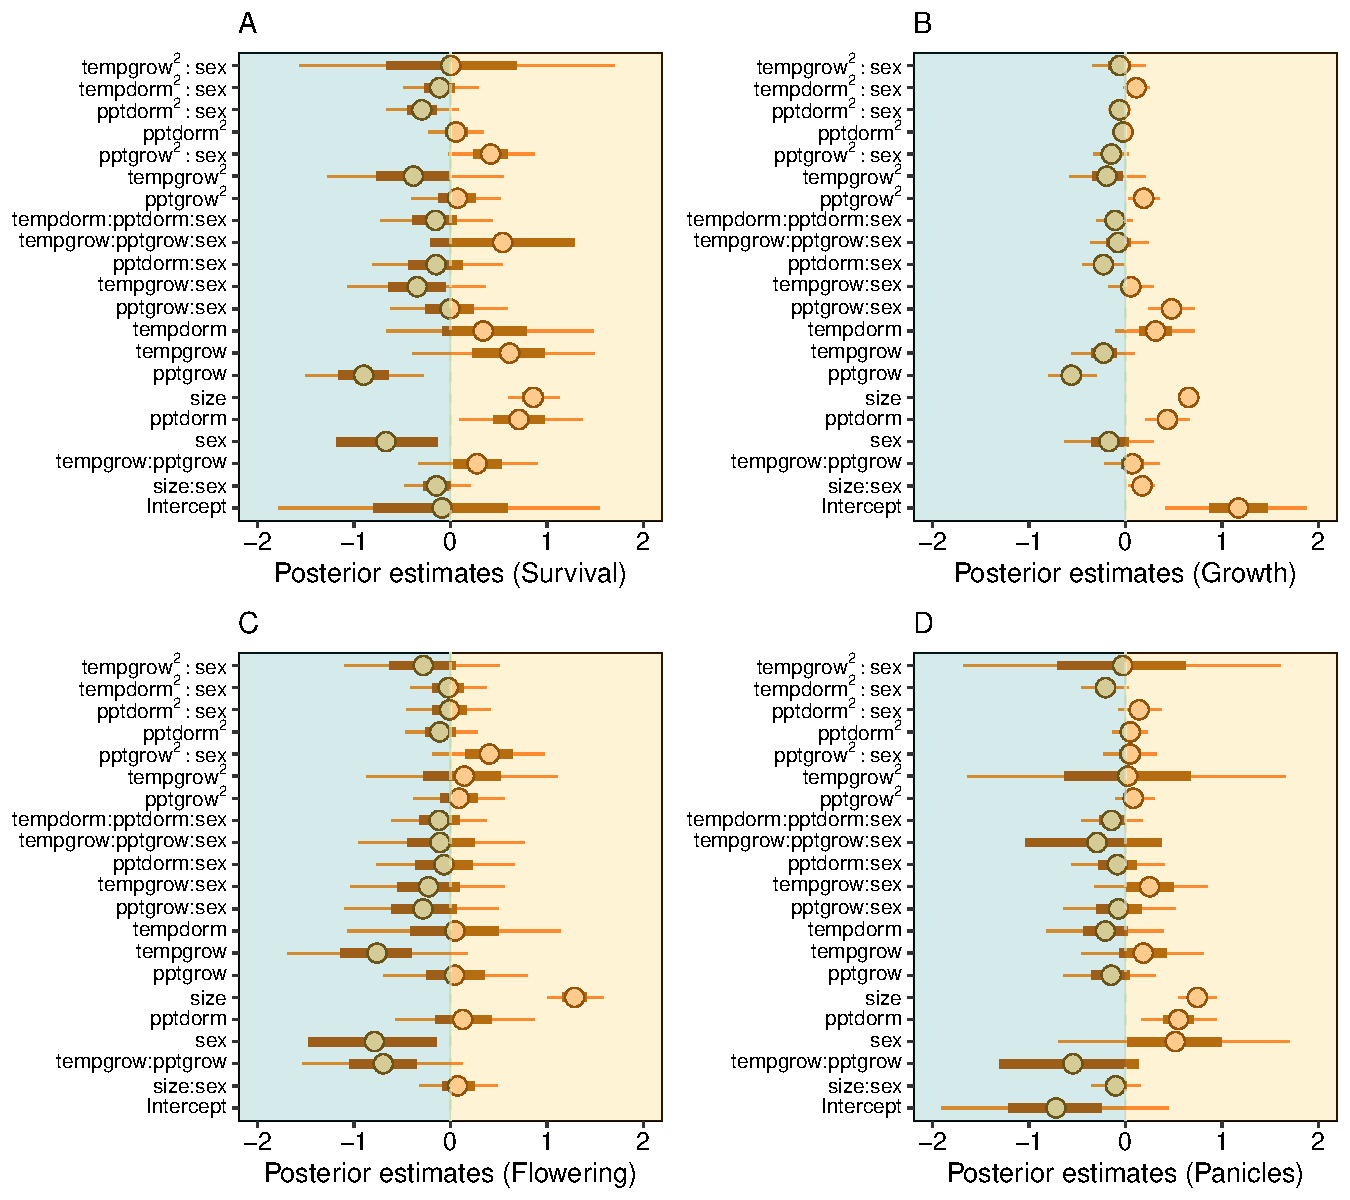
\includegraphics[width=0.95\linewidth]{Figures/Posterior_mean.pdf}
		\caption{Mean parameter values and 95\% credible intervals for all vital rates. 
		pptgrow is  the precipitation of growing season,
		Tempgrow is the temperature of growing season,
		pptdorm is the temperature of dormant season,
		Tempdorm is the temperature of dormant season.}
		\label{Sup:Posterior}
\end{figure}

\begin{figure}[H]
  \begin{center}
    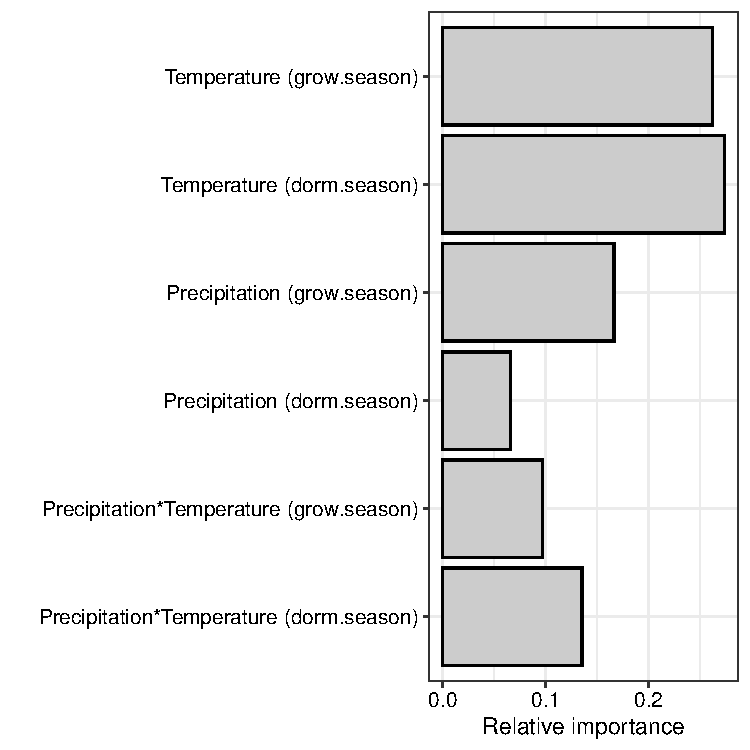
\includegraphics[width=0.65\linewidth]{Figures/Fig_LTRE.pdf}
  \caption{Life Table Response Experiment: The bar represent the relative importance of each predictors}
  \label{Sup:LTRE}
  \end{center}
\end{figure}

\begin{figure}[H]
  \begin{center}
    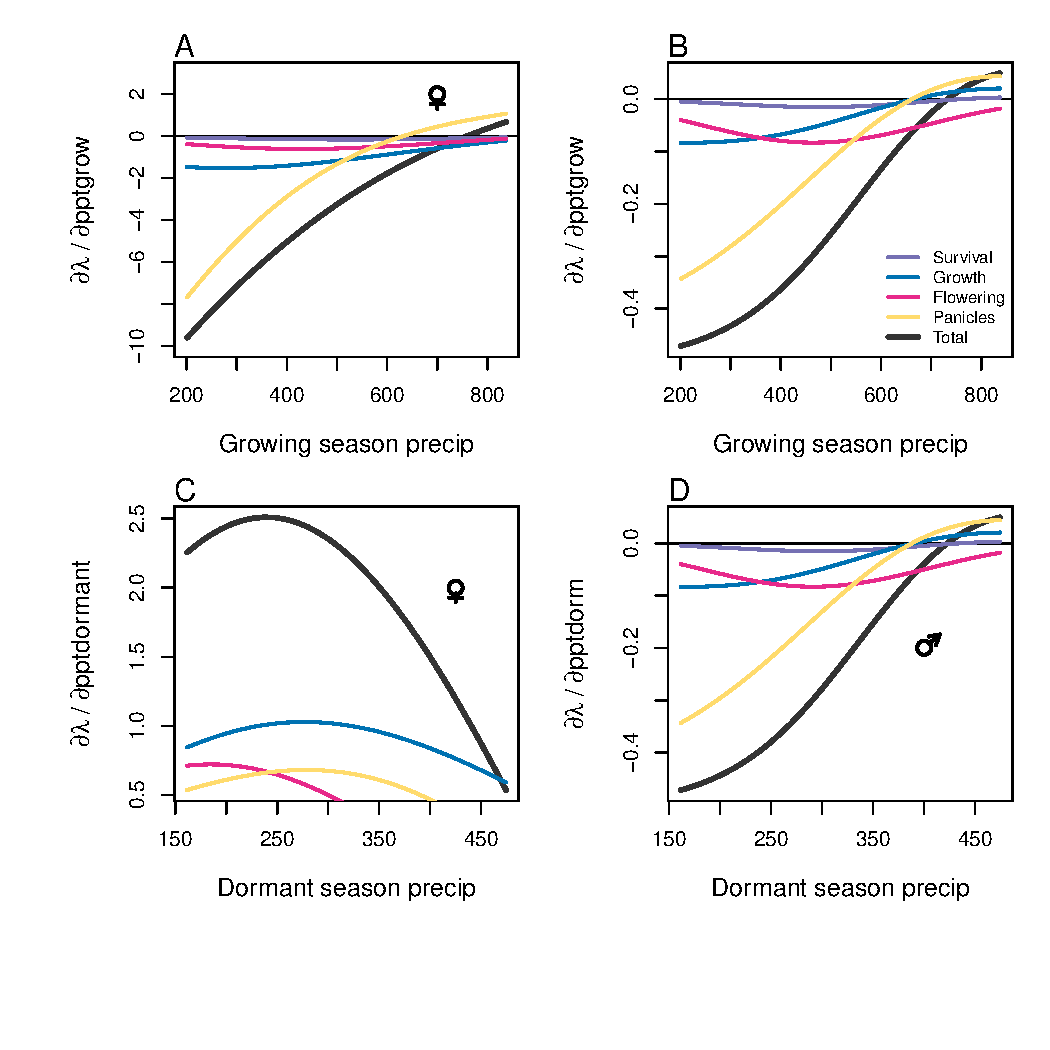
\includegraphics[width=0.98\linewidth]{Figures/LTRE_Precipitation.pdf}
  \caption{Life table response experiment decomposition of the sensitivity of $\lambda$ to seasonal climate into additive vital rate contributions of males and females based on posterior mean parameter estimates.
 (A) Precipitation of growing season (contribution of female), (B) Precipitation of growing season (contribution of male),  (C) Precipitation of dormant season (contribution of female) and (D) Precipitation of dormant season (contribution of male).}
  \label{Sup:LTRE_precip}
  \end{center}
\end{figure}

\begin{figure}[H]
  \begin{center}
    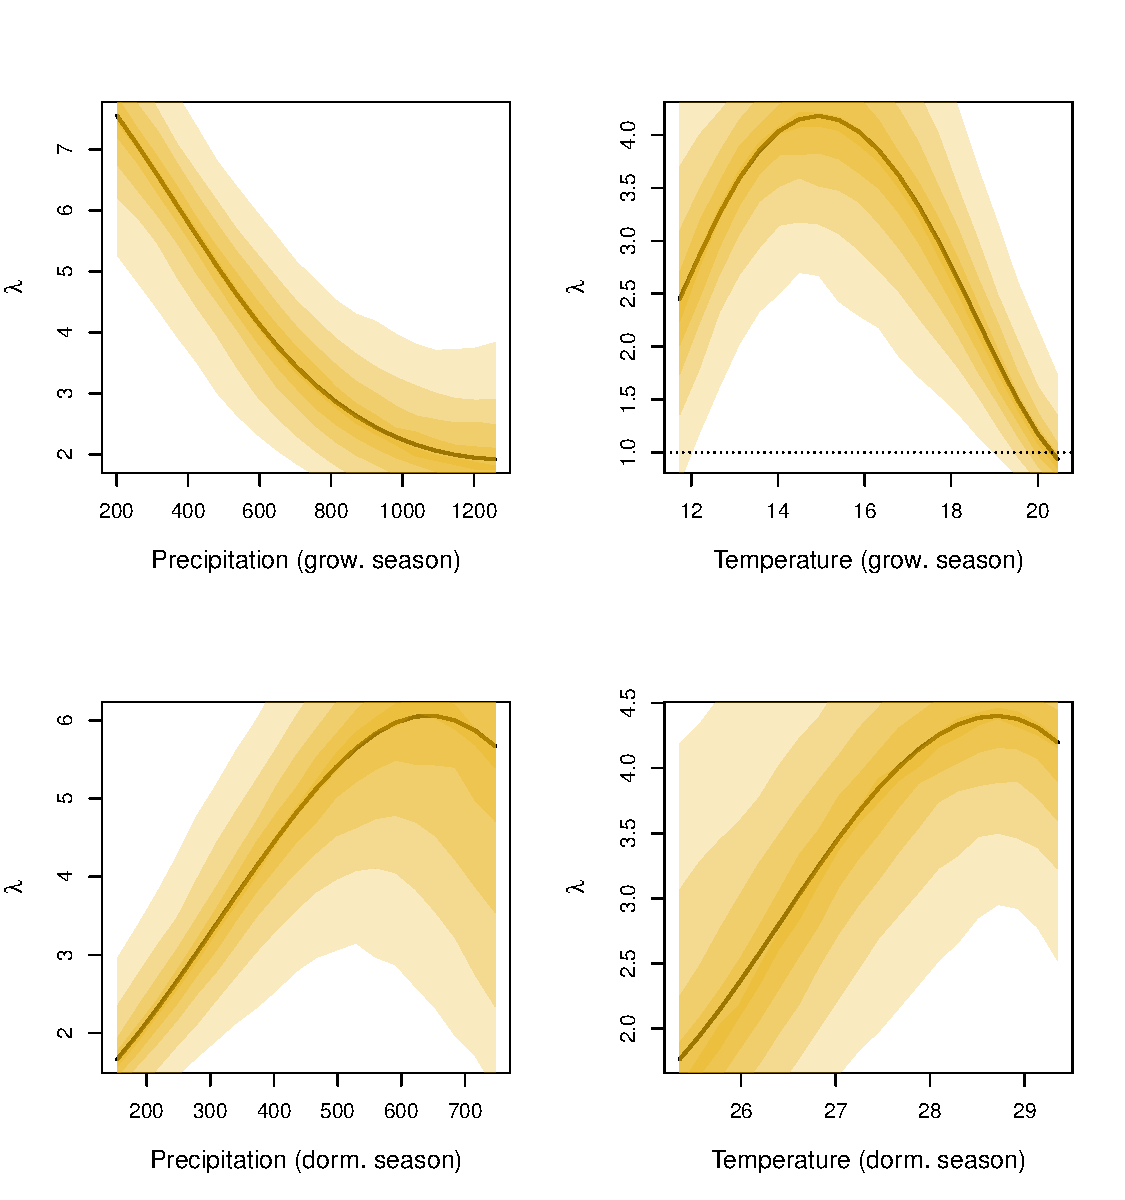
\includegraphics[width=0.95\linewidth]{Figures/lambda_CI.pdf}
  \caption{Population growth rate ($\lambda$) as a function of seasonal climate (2015-2017), predicted by the two-sex matrix projection model that incorporates sex-specific demographic responses to climate with sex ratio-dependent seed fertilization.
We show the mean posterior distribution of $\lambda$ in solid lines, and the 5, 25, 50, 75, and 95\% percentiles of parameter uncertainty in shaded gold color.
The dashed horizontal line indicates the limit of population viability ($\lambda$ = 1)}
  \label{Sup:lambda2sex}
  \end{center}
\end{figure}

\begin{figure}[H]
  \begin{center}
    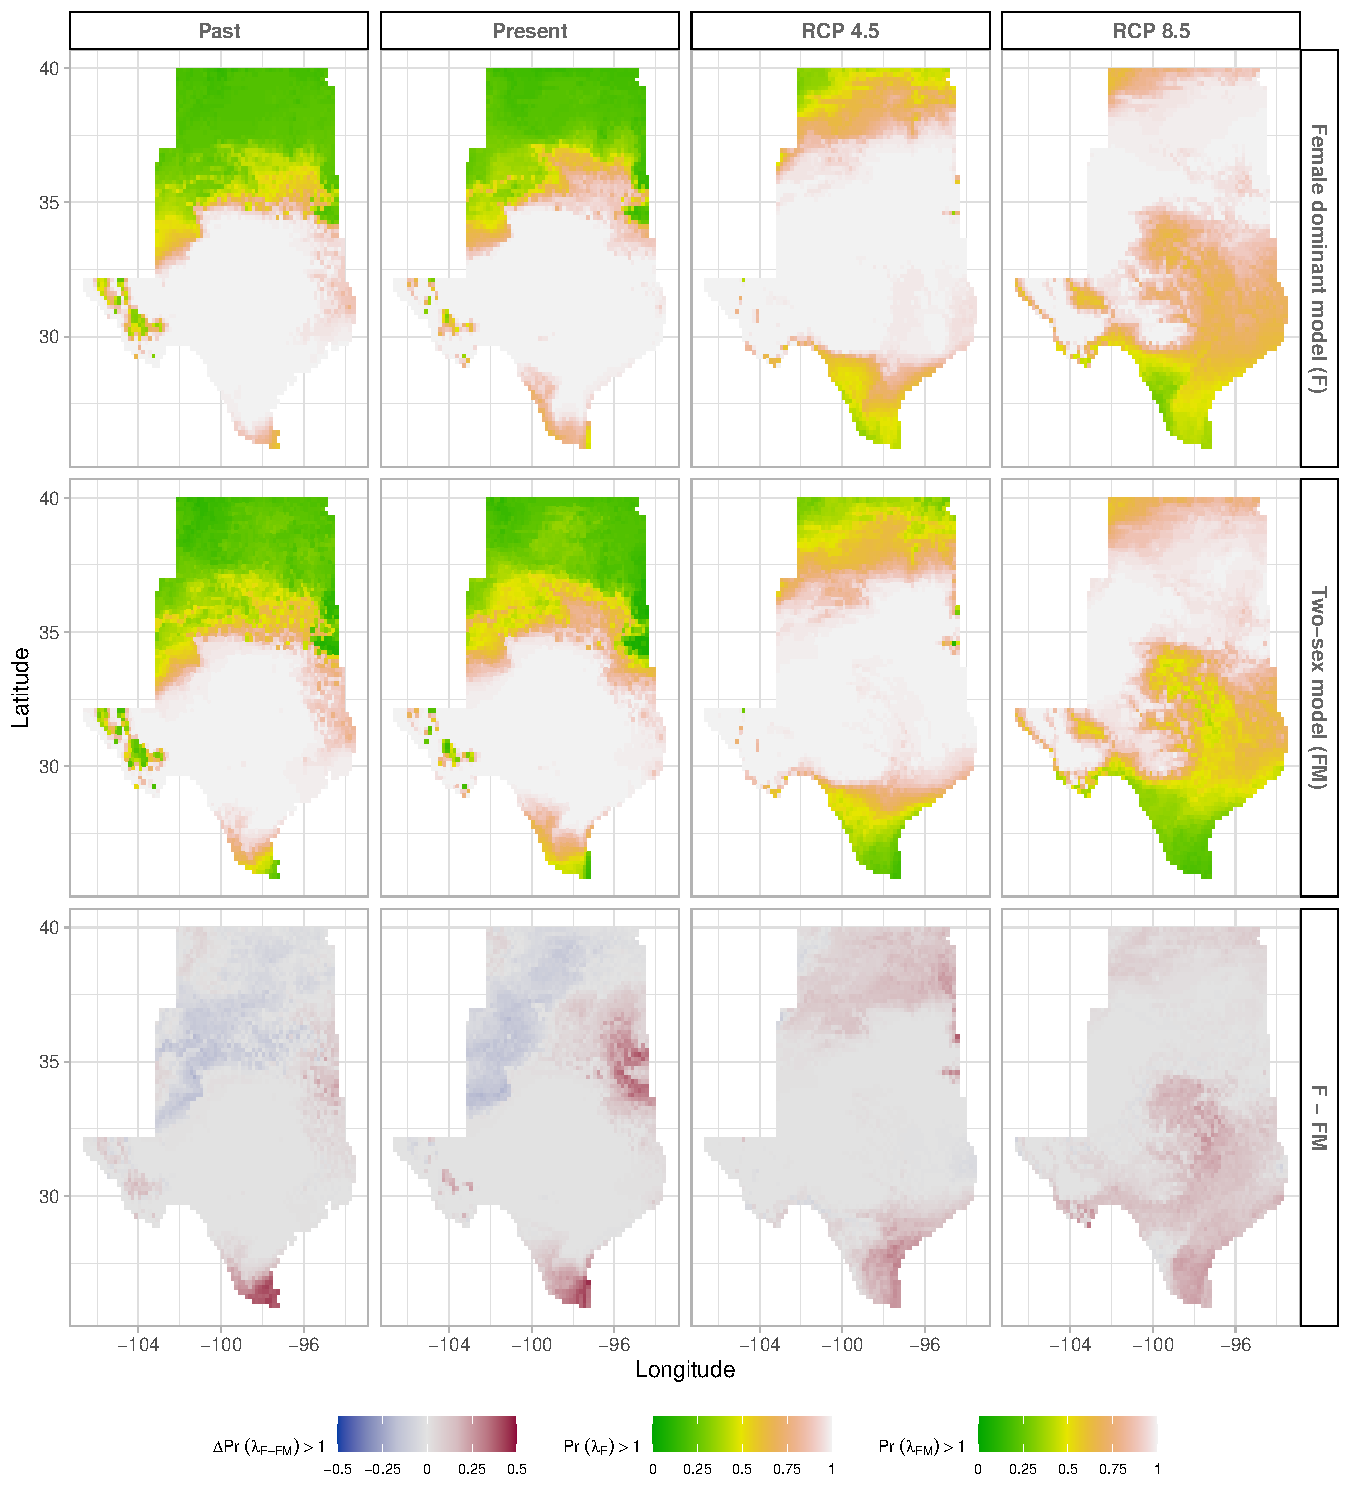
\includegraphics[width=0.95\linewidth]{Figures/Fig_geoPrlambda_ces.pdf}
  \caption{Climate change favors range shift toward the North edge of the current range.
  (A) Past, (B) Current, (C and D) Future predicted range shift based on the predicted probabilities of self- sustaining populations, Pr ($\lambda > 1$), using the two-sex model that incorporates sex- specific demographic responses to climate with sex ratio dependent seed fertilization.
  (E) Past, (F) Current, (G and F) Future  predicted range shift based on the predicted probabilities of self- sustaining populations, Pr ($\lambda > 1$), using the female dominant model.
  Future projections were based on the CESM1-BGC model.
  The black dots on panel B and F indicate all known presence points collected from GBIF from 1990 to 2019, which corresponds to the current condition in our prediction. 
  The occurrences of GBIFs are distributed in with higher population fitness habitat Pr ($\lambda$ > 1) , confirming that our study approach can reasonably predict range shifts. }
  \label{Sup:geoprojces}
  \end{center}
\end{figure}

\begin{figure}[H]
  \begin{center}
    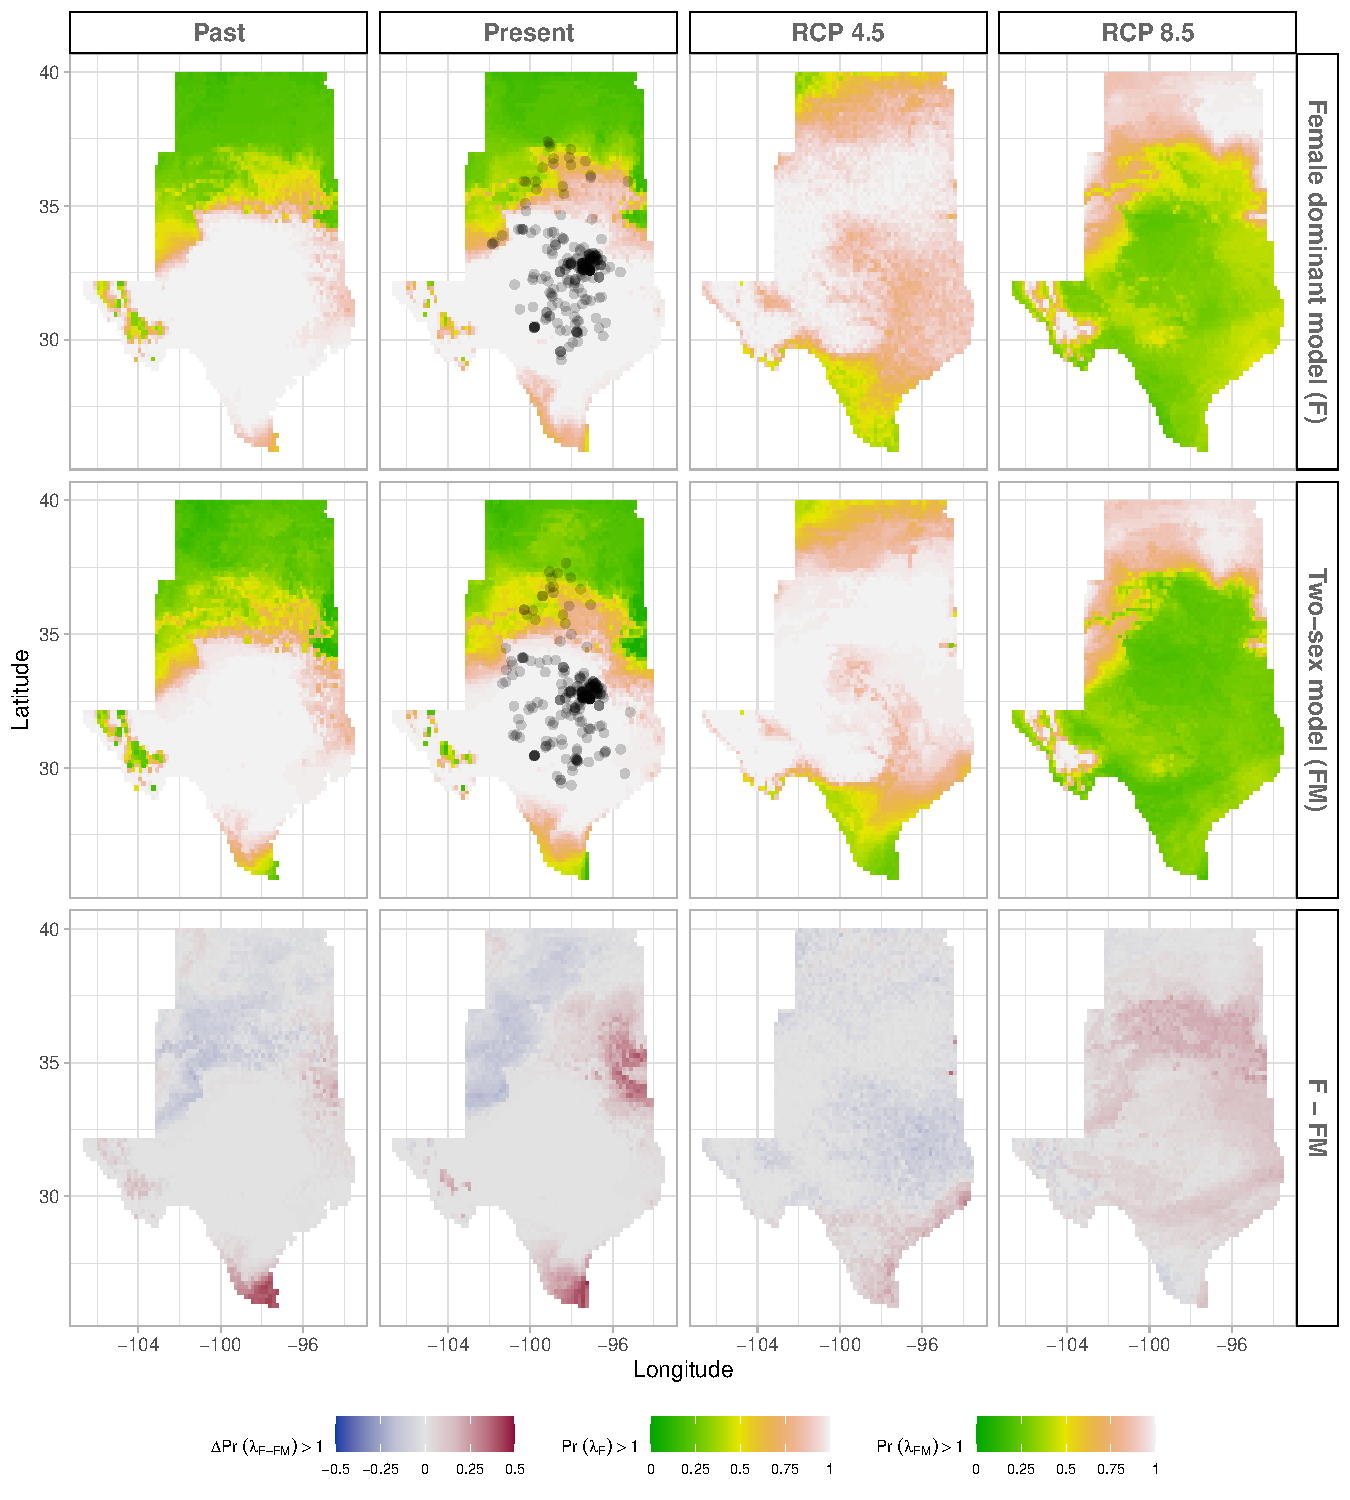
\includegraphics[width=0.95\linewidth]{Figures/Fig_geoPrlambdacmc.pdf}
  \caption{Climate change favors range shift toward the North edge of the current range.
  (A) Past, (B) Current, (C and D) Future predicted range shift based on the predicted probabilities of self- sustaining populations, Pr ($\lambda > 1$), using the two-sex model that incorporates sex- specific demographic responses to climate with sex ratio dependent seed fertilization.
  (E) Past, (F) Current, (G and F) Future  predicted range shift based on the predicted probabilities of self- sustaining populations, Pr ($\lambda > 1$), using the female dominant model.
  Future projections were based on the  CMCC-CM model.
  The black dots on panel B and F indicate all known presence points collected from GBIF from 1990 to 2019, which corresponds to the current condition in our prediction. 
  The occurrences of GBIFs are distributed in with higher population fitness habitat Pr ($\lambda$ > 1) , confirming that our study approach can reasonably predict range shifts.}
  \label{Sup:geoprojcmc}
  \end{center}
\end{figure}

\begin{figure}[H]
  \begin{center}
    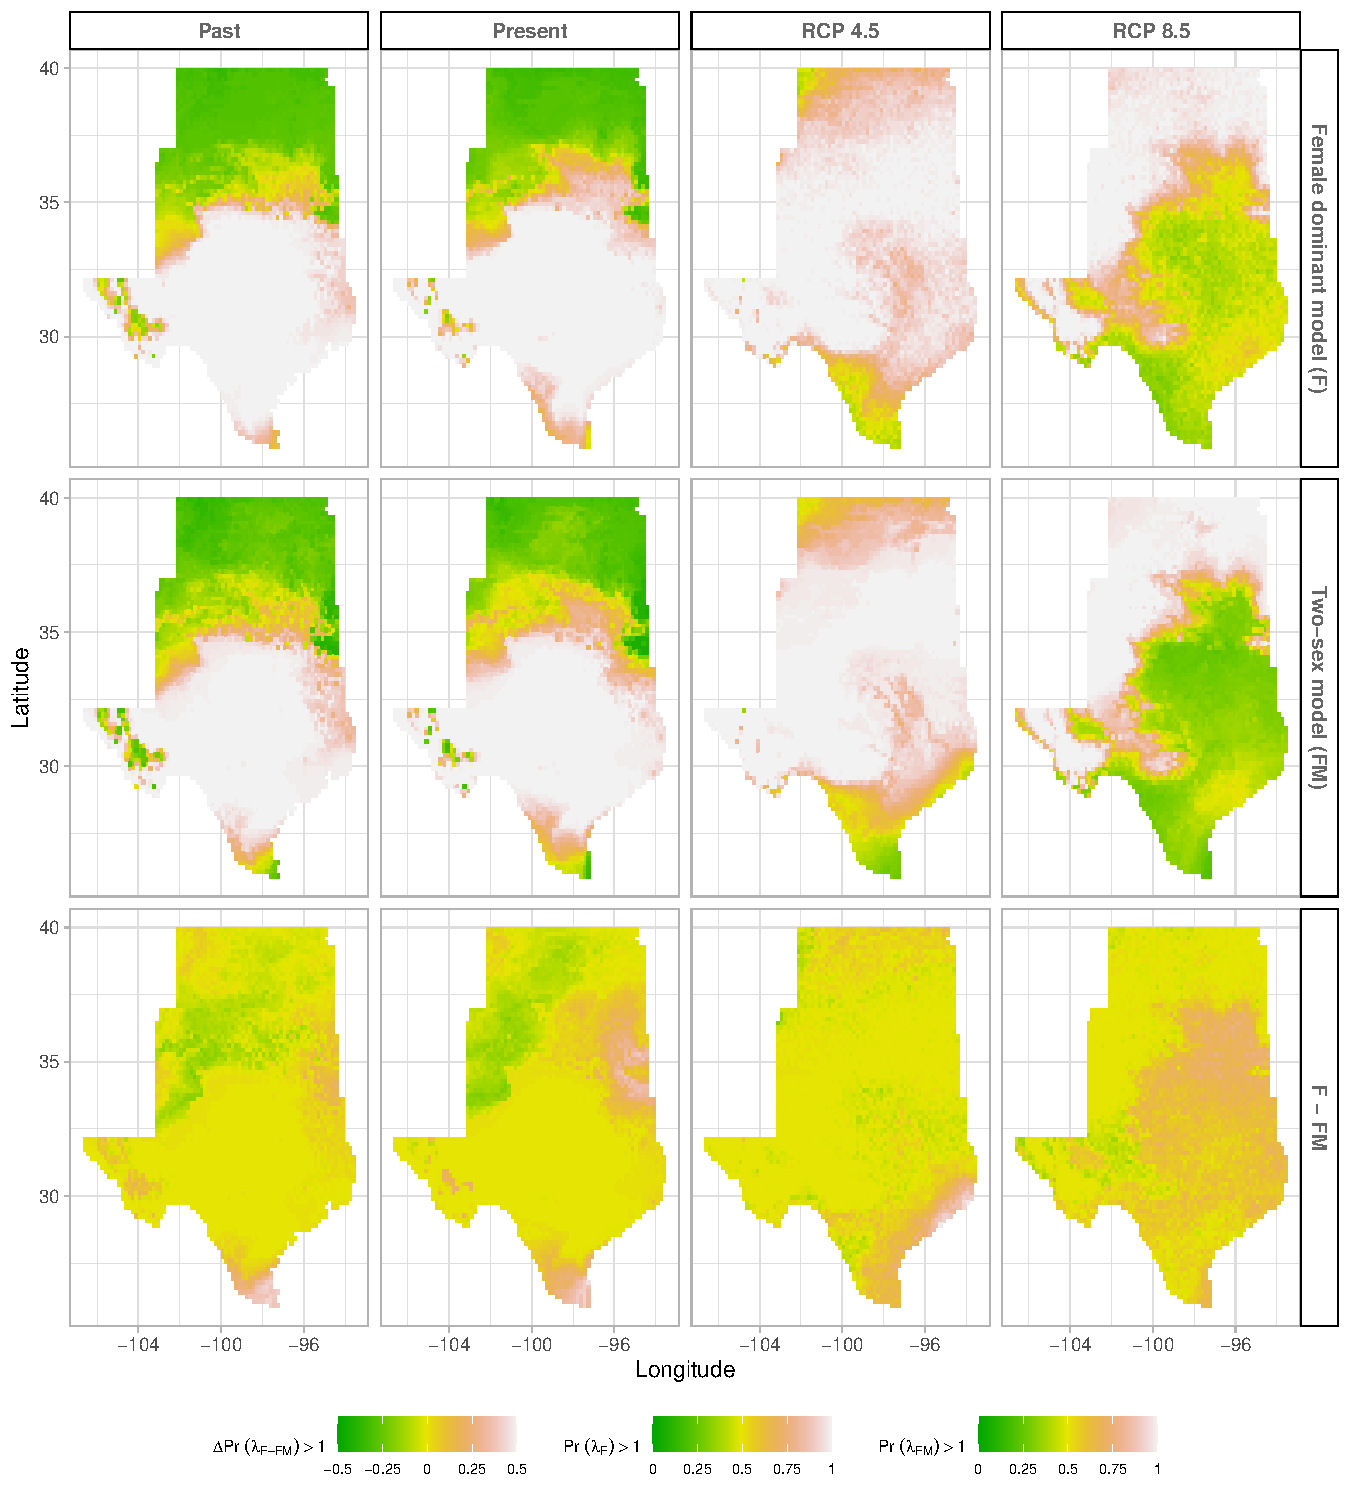
\includegraphics[width=0.95\linewidth]{Figures/Fig_geoPrlambda_miroc.pdf}
  \caption{Climate change favors range shift toward the North edge of the current range.
  (A) Past, (B) Current, (C and D) Future predicted range shift based on the predicted probabilities of self- sustaining populations, Pr ($\lambda > 1$), using the two-sex model that incorporates sex- specific demographic responses to climate with sex ratio dependent seed fertilization.
  (E) Past, (F) Current, (G and F) Future  predicted range shift based on the predicted probabilities of self- sustaining populations, Pr ($\lambda > 1$), using the female dominant model.
  Future projections were based on the MIROC5 model.
  The black dots on panel B and F indicate all known presence points collected from GBIF from 1990 to 2019, which corresponds to the current condition in our prediction. 
  The occurrences of GBIFs are distributed in with higher population fitness habitat Pr ($\lambda$ > 1) , confirming that our study approach can reasonably predict range shifts.}
  \label{Sup:geoprojmiroc}
  \end{center}
\end{figure}

\begin{figure}[H]
  \begin{center}
    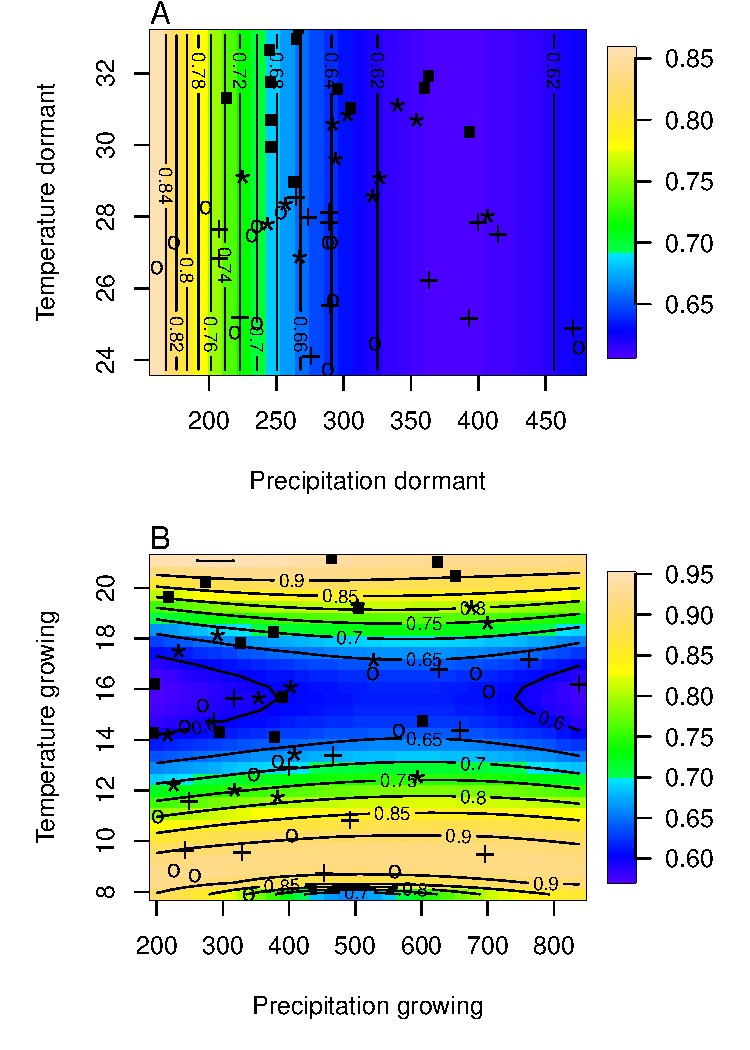
\includegraphics[width=0.75\linewidth]{Figures/OSR.pdf}
  \caption{A two‐dimensional representation of the Operational Sex Ratio (OSR) over time (past, present and future climate conditions). 
  OSR represents the proportion of females. 
  Contours show predicted values of OSR conditional on precipitation and temperature of the dormant and growing season.
  Operational Sex Ratio during the dormant season for the two sex model (A), Operational Sex Ratio during the growing season for the two sex model (B).
  "\begin{normalsize}\textbf{o}\end{normalsize}": Past, "\begin{normalsize}\textbf{+}\end{normalsize}": Current,"\begin{large}\textbf{*}\end{large}": RCP 4.5,"\begin{tiny}$\blacksquare$\end{tiny}": RCP 8.5.}
  \label{Sup:OSR}
  \end{center}
\end{figure}

% \begin{figure}[H]
%   \begin{center}
%     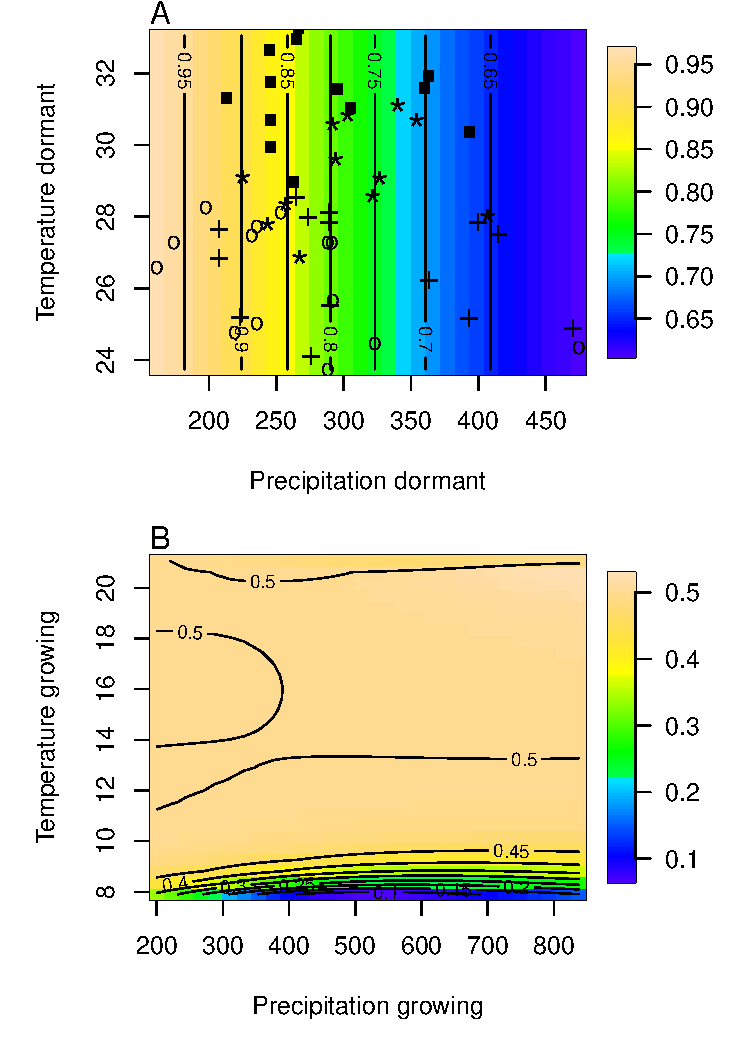
\includegraphics[width=0.85\linewidth]{Figures/SR.pdf}
%   \caption{A two‐dimensional representation of the  Sex Ratio (SR) over time (past, present and future climate conditions). 
%   Contours show predicted values of SR conditional on precipitation and temperature of the dormant and growing season.
%   Sex Ratio during the dormant season for the two sex model (A),Sex Ratio during the growing season for the two sex model (B).}
%   \label{Sup:SR}
%   \end{center}
% \end{figure}


\end{document}
